\documentclass[11pt,a4paper]{article}
\usepackage[utf8]{inputenc}
\usepackage{amsmath,amssymb,amsthm}
\usepackage{geometry}
\usepackage{booktabs}
\usepackage{tabularx}
\usepackage{hyperref}
\usepackage{microtype}
\usepackage{tikz}
\usepackage{pgfplots}
\pgfplotsset{compat=1.18}
\usetikzlibrary{arrows,positioning,shapes.geometric,calc}

\geometry{margin=1in}

\hypersetup{
    colorlinks=true,
    linkcolor=blue,
    citecolor=blue,
    urlcolor=blue,
    pdftitle={Mathematical Foundations of the Direct Acyclic Validation \& Inference Engine (DAVID/M0.1)},
    pdfauthor={Arben Lila}
}

\newtheorem{theorem}{Theorem}
\newtheorem{lemma}[theorem]{Lemma}
\newtheorem{definition}{Definition}
\newtheorem{claim}[theorem]{Claim}
\newtheorem{critique}{Critique}
\newtheorem{defense}{Defense}
\newtheorem{remark}{Remark}

\title{\textbf{Mathematical Foundations of the Direct Acyclic Validation \& Inference Engine (DAVID/M0.1)}\\
\large A Gated Predictive Architecture for Latent Regime Dynamics under Multi-Source Information-Theoretic Gating}
\author{\textbf{Arben Lila} \\ \textit{Internal Thesis Work}}
\date{\today}

\begin{document}

\maketitle

\begin{abstract}
This document establishes the complete, self-contained mathematical foundations of the Direct Acyclic Validation \& Inference Engine (DAVID) version M0.1. Unlike traditional un-gated statistical predictors, the DAVID engine introduces the paradigm of \textit{Gated Predictive Claims}, where conditional forecasts are treated as formal claims that must pass a sequence of rigorous information-theoretic firewalls. We present detailed, step-by-step mathematical proofs for the four core theorems governing these gates: (i) Theorem $A'$ concerning source-channel latent-class identifiability under Kruskal tensor rank constraints; (ii) Theorem $B'$ establishing single-observation Bayes classification error bounds and the quadratic scaling of Fisher Information; (iii) Theorem $C$ establishing dependency-robust posterior expected FDP control --- valid under arbitrary spatial and temporal dependence among the latent activity variables, conditional on valid posterior probabilities; and (iv) Theorem $D$-forecast establishing ergodic convergence of dwell-age-aware Hidden Semi-Markov Model (HSMM) forecasts to the time-weighted stationary law, which underwrites an operational horizon diagnostic $h^\star$. % %%NEEDS_HUMAN_MATH_REVIEW%% Furthermore, we expose each theorem to adversarial mathematical critiques from the perspective of a leading statistician in the field and construct formal defenses and implementation-level mitigations for each challenge, ensuring the scientific defensibility of the engine under real-world failures.
\end{abstract}

\tableofcontents
\newpage

\section{Introduction \& The Gated Predictor Innovation}
Traditional forecasting models in public policy, epidemiology, and economics operate under an "always-emit" paradigm. Given any historical sequence of inputs, these systems generate point forecasts and confidence intervals, regardless of whether the underlying latent states are identifiable, the data channels are informative, or the forecast horizon has decayed completely into the stationary prior. This un-gated approach leads to three critical pathologies:
\begin{enumerate}
    \item \textbf{Statistical Hallucinations:} Emitting precise-looking point estimates from data that lies in the unidentifiable singular region of the parameter space.
    \item \textbf{Prior Domination:} Emitting predictions from highly noisy channels that are driven entirely by prior assumptions rather than empirical evidence, misleading decision-makers into false confidence.
    \item \textbf{Ergodic Memory Loss:} Emitting conditional forecasts far into the future where transition noise has completely erased the memory of the current state, producing predictions that simply "predict the stationary prior" under the guise of dynamic forecasts.
\end{enumerate}

The core architectural innovation of the \textbf{Direct Acyclic Validation \& Inference Engine (DAVID)} is the concept of a \textbf{Gated Predictive Claim}. Instead of treating forecasting as a direct mapping from estimation to output, the engine wraps the posterior distribution in a nested stack of mathematical firewalls. If any gate is violated, the forecast "fail-closes" honestly, degrading to a safe, uninformative state (e.g., an evidence-gap flag, a wide prior interval, or the stationary marginal prior).

This document details the complete mathematical formulation of these gates, provides step-by-step proofs for their underlying theorems, and subjects them to rigorous mathematical challenges and defenses.

---

\section{Theorem $A'$ --- Source-Channel Latent-Class Identifiability}

\subsection{Setting and Measurement Architecture}
Within a specific policy stratum $g$ (defined by a country and a policy area, e.g., the Kosovo Smoke-Free policy stratum), the engine distinguishes \textbf{two measurement layers} that must not be conflated:
\begin{enumerate}
    \item \textbf{Layer 1 (source detection).} $S$ detection channels $s = 1, \dots, S$ --- web scrapers, media feeds, and institutional report streams --- each searching for evidence of the latent activity through a separate acquisition pipeline. The identification argument of this section applies to this layer only. % %%NEEDS_HUMAN_MATH_REVIEW%%
    \item \textbf{Layer 2 (coder reliability).} $M$ LLM coders that read the \emph{same} retrieved document for a given unit and emit binary labels. Because all coders condition on a common document, their errors are conditionally dependent given the latent activity; they therefore enter the likelihood through a separate Dawid--Skene coder-reliability layer (sensitivity $\kappa^+_m$ and specificity $\kappa^-_m$ per coder $m$, calibrated against gold adjudicated labels) and are \emph{not} counted among the $S$ sources. The implemented model (\texttt{m01\_forward.stan}) maintains exactly this separation: $(\rho_s, \delta_s)$ per source, $(\kappa^+_m, \kappa^-_m)$ per coder. % %%NEEDS_HUMAN_MATH_REVIEW%%
\end{enumerate}

Identifiability is a property of a \emph{population} joint law; it therefore requires replication. Within stratum $g$ we observe units $u = 1, \dots, N_g$ (e.g., month--tactic detection opportunities), with latent activity indicators and source labels
\[
A_{g,u} \overset{\text{iid}}{\sim} \mathrm{Bernoulli}(\phi), \qquad Y_{s,u} \in \{0,1\}, \quad s = 1, \dots, S. % %%NEEDS_HUMAN_MATH_REVIEW%%
\]
Each source $s \in \{1, \dots, S\}$ is characterized by its channel parameters:
\begin{align*}
    \text{Sensitivity (True Positive Rate):} \quad \rho_s &= P(Y_{s,u} = 1 \mid A_{g,u} = 1) \\
    \text{False Positive Rate:} \quad \delta_s &= P(Y_{s,u} = 1 \mid A_{g,u} = 0)
\end{align*}
We state the maintained assumptions explicitly:
\begin{itemize}
    \item[(A1)] \textbf{Replication.} The units $u = 1, \dots, N_g$ are i.i.d.\ draws from the stratum law, so the empirical joint distribution of $(Y_{1,u}, \dots, Y_{S,u})$ converges to the population law $P(Y_1, \dots, Y_S)$ as $N_g \to \infty$. When units are time-indexed and serially dependent (the HSMM regime layer), (A1) is relaxed to stationarity and ergodicity within a regime segment; the empirical law still converges, but the effective replication count is reduced as quantified in the dependent-sample analysis accompanying Theorem $B'$. % %%NEEDS_HUMAN_MATH_REVIEW%%
    \item[(A2)] \textbf{Conditional independence across sources.} $P(Y_{1,u}, \dots, Y_{S,u} \mid A_{g,u}) = \prod_{s=1}^{S} P(Y_{s,u} \mid A_{g,u})$. % %%NEEDS_HUMAN_MATH_REVIEW%%
    \item[(A3)] \textbf{Channel homogeneity.} $(\rho_s, \delta_s)$ are constant across units within the stratum. % %%NEEDS_HUMAN_MATH_REVIEW%%
\end{itemize}
The observed data is the empirical joint law of $(Y_1, \dots, Y_S)$ accumulated over the $N_g$ replicates. We must guarantee that $\theta = (\phi, \{\rho_s, \delta_s\}_{s=1}^S)$ is uniquely determined by the population law $P(Y_1, \dots, Y_S)$. A single unit --- or a single unreplicated sequence --- does \emph{not} identify $\theta$: identification is a statement about the law, and the law is estimable only under replication (A1). The Allman--Matias--Rhodes (2009) framework invoked below is likewise a statement about the population joint law. % %%NEEDS_HUMAN_MATH_REVIEW%%

\subsection{Formal Statement}
\begin{theorem}[Latent-Class Identifiability]
Assume (A1)--(A3). Then the parameters $\phi$ and $\{\rho_s, \delta_s\}_{s=1}^{S}$ of the 2-class product-Bernoulli latent class model are identifiable from the population joint law $P(Y_1, \dots, Y_S)$, uniquely up to the single simultaneous swap % %%NEEDS_HUMAN_MATH_REVIEW%%
\[
(\phi, \{\rho_s\}, \{\delta_s\}) \;\longmapsto\; (1 - \phi, \{\delta_s\}, \{\rho_s\}), % %%NEEDS_HUMAN_MATH_REVIEW%%
\]
provided that:
\begin{enumerate}
    \item At least $S \ge 3$ sources are observed;
    \item At least three effective independent source views satisfy $\rho_s \neq \delta_s$ (non-degenerate channels), and these three views identify $\phi$ together with their own channel parameters $\{(\rho_s, \delta_s)\}$. Additional degenerate channels satisfying $\rho_s = \delta_s$ may be present as nuisance channels; they are identifiable only under that constraint, in which case their common Bernoulli rate $q_s = \rho_s = \delta_s$ is identified from the marginal distribution $P(Y_s)$; they do not contribute to the Kruskal rank condition or headline identification claims; % %%NEEDS_HUMAN_MATH_REVIEW%%
    \item The prior probability is non-boundary: $\phi \in (0, 1)$.
\end{enumerate}
Identifiability holds at \emph{every} parameter point satisfying conditions 1--3, not merely generically: conditions 2--3 exactly delimit the singular set excluded by the Kruskal rank condition used in the proof. The residual label swap is removed by the orientation convention $\rho_s > \delta_s$, which the implementation enforces by construction (the Stan parameterization sets $\rho_s = \delta_s + (1 - \delta_s)\,\mathrm{logit}^{-1}(j_s)$ with $j_s$ finite, so $\rho_s > \delta_s$ almost surely). The inequality $\rho_s > \delta_s$ orients the statistical class (the high-detection-probability regime); substantive interpretation of this class as industry interference activity requires external positive and negative anchor units calibrated by human adjudication. % %%NEEDS_HUMAN_MATH_REVIEW%%
\end{theorem}

\subsection{Step-by-Step Proof}
\begin{proof}
Let $S = 3$; the case $S > 3$ is handled at the end by marginalization. Under (A2), the population joint distribution of $Y_1, Y_2, Y_3$ is the three-way tensor $T \in \mathbb{R}^{2 \times 2 \times 2}$ with
\begin{equation}\label{eq:tensor_cp}
T_{ijk} = P(Y_1=i, Y_2=j, Y_3=k) = \sum_{a \in \{0, 1\}} \pi_a M^{(1)}_{ia} M^{(2)}_{ja} M^{(3)}_{ka}
\end{equation}
Here, $\pi_1 = \phi$, $\pi_0 = 1 - \phi$, and the factor matrices $M^{(s)} \in \mathbb{R}^{2 \times 2}$ are defined by:
\[
M^{(s)} = \begin{pmatrix} P(Y_s=0 \mid A=0) & P(Y_s=0 \mid A=1) \\ P(Y_s=1 \mid A=0) & P(Y_s=1 \mid A=1) \end{pmatrix} = \begin{pmatrix} 1-\delta_s & 1-\rho_s \\ \delta_s & \rho_s \end{pmatrix}
\]
for $s \in \{1, 2, 3\}$. Equation~\eqref{eq:tensor_cp} is a Canonical Polyadic (CP) decomposition of $T$ into $R = 2$ rank-1 terms, with strictly positive weights $\pi_0, \pi_1 > 0$ by condition 3; positivity of both weights is required for the application of Kruskal's theorem below (a zero weight collapses the decomposition to rank 1). % %%NEEDS_HUMAN_MATH_REVIEW%%

According to \textbf{Kruskal's Uniqueness Theorem} (Kruskal, 1977), the CP decomposition of a 3-way tensor into $R$ rank-1 terms with nonzero weights is unique up to permutation and rescaling of the rank-1 factors if:
\begin{equation}\label{eq:kruskal_bound_formula}
k(M^{(1)}) + k(M^{(2)}) + k(M^{(3)}) \ge 2R + 2
\end{equation}
where $k(M^{(s)})$ is the Kruskal rank (or $k$-rank) of matrix $M^{(s)}$, defined as the largest integer $k$ such that any $k$ columns of $M^{(s)}$ are linearly independent.

Since each $M^{(s)}$ is of size $2 \times 2$, it contains exactly 2 columns. The columns are linearly independent (implying $k(M^{(s)}) = 2$) if and only if the matrix has full rank, which holds if and only if its determinant is non-zero:
\[
\det(M^{(s)}) = (1-\delta_s)\rho_s - (1-\rho_s)\delta_s = \rho_s - \delta_s
\]
By assumption (condition 2), at least three effective independent source views satisfy $\rho_s \neq \delta_s$; choose any such triple $(s_1, s_2, s_3)$. For each chosen $s_i$, $\det(M^{(s_i)}) = \rho_{s_i} - \delta_{s_i} \neq 0$. (Any additional sources need not be non-degenerate; degenerate nuisance sources are excluded from this triple and do not affect the rank argument.) Thus: % %%NEEDS_HUMAN_MATH_REVIEW%%
\[
k(M^{(1)}) = k(M^{(2)}) = k(M^{(3)}) = 2
\]
Summing the Kruskal ranks of the three factor matrices:
\[
k(M^{(1)}) + k(M^{(2)}) + k(M^{(3)}) = 2 + 2 + 2 = 6
\]
For $R=2$ latent classes, the right-hand side of Equation~\eqref{eq:kruskal_bound_formula} is:
\[
2R + 2 = 2(2) + 2 = 6
\]
Since $6 \ge 6$, Kruskal's uniqueness condition is satisfied: the CP decomposition of $T$ into two rank-1 terms is unique up to (i) rescaling within each component and (ii) permutation of the two components (Kruskal, 1977; applied to latent-class structures by Allman--Matias--Rhodes, 2009). Both indeterminacies are resolved in the probabilistic setting: % %%NEEDS_HUMAN_MATH_REVIEW%%
\begin{itemize}
    \item \textbf{Scaling.} Each column of each $M^{(s)}$ is a conditional probability mass function and must sum to 1, and the weights must satisfy $\pi_0 + \pi_1 = 1$; this fixes the scale of every factor exactly. % %%NEEDS_HUMAN_MATH_REVIEW%%
    \item \textbf{Permutation.} The remaining ambiguity is the single simultaneous swap of the two latent classes, $(\phi, \{\rho_s\}, \{\delta_s\}) \mapsto (1-\phi, \{\delta_s\}, \{\rho_s\})$, exactly as asserted in the theorem statement; it is removed by the orientation convention $\rho_s > \delta_s$. % %%NEEDS_HUMAN_MATH_REVIEW%%
\end{itemize}

It remains to rule out alternative parameters \emph{outside} the constrained set, i.e., a degenerate $\theta'$ (with $\phi' \in \{0, 1\}$, or some $\rho'_s = \delta'_s$) reproducing the same law, since Kruskal's theorem compares only decompositions of the stated rank. Under conditions 1--3, every pairwise covariance is nonzero: % %%NEEDS_HUMAN_MATH_REVIEW%%
\[
\mathrm{Cov}(Y_s, Y_{s'}) = \phi(1 - \phi)(\rho_s - \delta_s)(\rho_{s'} - \delta_{s'}) \neq 0 \qquad (s \neq s'). % %%NEEDS_HUMAN_MATH_REVIEW%%
\]
Any $\theta'$ with $\phi' \in \{0, 1\}$ makes all sources mutually independent (all pairwise covariances zero), and any $\theta'$ with $\rho'_s = \delta'_s$ makes source $s$ independent of the others ($\mathrm{Cov}(Y_s, Y_{s'}) = 0$ for all $s'$). Neither can reproduce $T$. Hence no degenerate alternative exists, and identifiability holds at every interior parameter point. % %%NEEDS_HUMAN_MATH_REVIEW%%

For $S > 3$, apply the result to the triple $(Y_1, Y_2, Y_3)$ to identify $\phi$ and channels 1--3, then to each triple $(Y_1, Y_2, Y_s)$, $s \ge 4$, to identify channel $s$; the latent-class orientation is aligned across triples because the shared channels 1 and 2 have $\rho \neq \delta$, making the matching of components across triples unambiguous. % %%NEEDS_HUMAN_MATH_REVIEW%%

Finally, we emphasize the role of (A1): Theorem $A'$ determines $\theta$ from the \emph{population} law $P(Y_1, \dots, Y_S)$; the empirical law converges to it only across replicated units $u = 1, \dots, N_g$. A single realization of $(Y_1, \dots, Y_S)$ carries at most 3 bits and cannot determine a 7-dimensional parameter; without replication the theorem makes no finite-sample claim whatsoever. % %%NEEDS_HUMAN_MATH_REVIEW%%
\end{proof}

\subsection{Degrees-of-Freedom Heuristic ($S=2$ vs $S=3$): Necessary, Not Sufficient}
Comparing the number of independent equations (observable cell probabilities) to the number of unknowns (parameters) is a useful \emph{negative} diagnostic. It must not be mistaken for an identifiability proof: equal counts are a necessary condition for identifiability, never a sufficient one. % %%NEEDS_HUMAN_MATH_REVIEW%%

\subsubsection{The Case of $S=2$ Sources (Unidentifiable)}
With two binary sources $Y_1, Y_2$, the joint probability table contains $2^2 = 4$ cells. Since the probabilities must sum to 1, we have $4 - 1 = \textbf{3}$ independent equations.
We are trying to estimate:
\begin{itemize}
    \item The prior: $\phi$ (1 parameter)
    \item Channel 1: $\rho_1, \delta_1$ (2 parameters)
    \item Channel 2: $\rho_2, \delta_2$ (2 parameters)
\end{itemize}
This results in \textbf{5 unknowns}. A continuous map from a 5-dimensional parameter space into a 3-dimensional moment space cannot be injective: the preimage of the observed law is (generically) a 2-dimensional manifold of indistinguishable parameters. Here counting delivers a valid \emph{impossibility} result, because matching dimensions is necessary for identifiability. % %%NEEDS_HUMAN_MATH_REVIEW%%

\subsubsection{The Case of $S=3$ Sources (No Dimension Obstruction --- Uniqueness from Kruskal Only)}
With three binary sources, the joint table has $2^3 = 8$ cells, providing $8 - 1 = \textbf{7}$ independent equations against \textbf{7 unknowns} ($\phi$ plus three channel pairs). Equal counts show only that there is no dimension obstruction. They do \emph{not} establish uniqueness: % %%NEEDS_HUMAN_MATH_REVIEW%%
\begin{itemize}
    \item The label swap $(\phi, \{\rho_s\}, \{\delta_s\}) \mapsto (1-\phi, \{\delta_s\}, \{\rho_s\})$ produces two distinct solutions of the same 7-equation system for \emph{every} law generated by the model --- a finite ambiguity invisible to any dimension count. % %%NEEDS_HUMAN_MATH_REVIEW%%
    \item Counting is insensitive to rank degeneracy. If one source is degenerate ($\rho_3 = \delta_3$), the count is still $7 = 7$, yet $Y_3$ is independent of $A$, the system collapses to the unidentifiable $S = 2$ case plus an independent Bernoulli nuisance, and the solution set containing the truth becomes positive-dimensional. % %%NEEDS_HUMAN_MATH_REVIEW%%
    \item In general, a polynomial system with as many equations as unknowns may have one solution, many isolated solutions, or a continuum on degenerate subsets; which case obtains is a rank question, not a counting question. % %%NEEDS_HUMAN_MATH_REVIEW%%
\end{itemize}
The uniqueness guarantee for $S = 3$ is supplied solely by \textbf{Kruskal's theorem (1977)} through the rank condition $\sum_s k(M^{(s)}) \ge 2R + 2$, verified in the proof above. The counting argument is retained only as intuition for why $S = 3$ is the minimal source count at which identification becomes \emph{possible}. % %%NEEDS_HUMAN_MATH_REVIEW%%

\subsection{Operational Diagnostic}
Theorem $A'$ is a population statement assuming (A1)--(A3) and an infinite-sample joint law. Near the singular set --- where some $\rho_s \approx \delta_s$, or $\phi \approx 0$ or $1$ --- the parameters remain formally identifiable, but the map from the observed law to the parameters becomes ill-conditioned and finite-sample posteriors degenerate. To control this, the engine calculates the \textbf{practical identification distance} $d(\theta)$ for each MCMC draw:
\[
d(\theta) = \min \left( J_{(3)}, \;\; \min(\phi,\, 1 - \phi) \right) % %%NEEDS_HUMAN_MATH_REVIEW%%
\]
where $J_{(3)}$ denotes the \emph{third-largest} Youden index: sort the per-source values $J_s = |\rho_s - \delta_s|$ in descending order and take the third. When $S < 3$ the stratum is under-sourced and the conventional $\min_s J_s$ is used as a conservative fallback (the gate will fail on $d(\theta)$ regardless, since the Kruskal rank condition is unmet). % %%NEEDS_HUMAN_MATH_REVIEW%%
\begin{itemize}
    \item The source-layer term $J_{(3)}$ matches the identifiability theorem: Kruskal's condition requires three independent informative views, not all $S$. Using $\min_s J_s$ would disqualify an identified stratum merely because one weak nuisance source is included. $J_{(3)}$ vanishes if and only if fewer than three source families satisfy $\rho_s \neq \delta_s$, which is the correct boundary. We emphasize that $\rho_s = 1 - \delta_s$ is \emph{not} a non-identification boundary: the symmetric channel $(\rho_s, \delta_s) = (0.9, 0.1)$ lies on it, has $J_s = 0.8$, and is highly informative. An earlier draft included a $|\rho_s - (1 - \delta_s)|$ term in $d(\theta)$, which incorrectly penalized the best channels; it has been removed. % %%NEEDS_HUMAN_MATH_REVIEW%%
    \item The $\min(\phi, 1 - \phi)$ term guards the class-balance boundary: as $\phi \to \{0, 1\}$ one latent class becomes vanishingly rare, the information about that class's channel parameters in any finite sample tends to zero, and practical identification fails even though $\phi \in (0, 1)$ formally satisfies condition 3. % %%NEEDS_HUMAN_MATH_REVIEW%%
\end{itemize}
\textbf{What $d(\theta) \ge 0.05$ does and does not certify.} $d(\theta)$ is a \emph{within-model} distance to the singular set, computed from the fitted posterior. Its validity as a diagnostic presumes (A1)--(A3) and a correctly specified likelihood. If conditional independence (A2) fails, the posterior may concentrate on a pseudo-true parameter with large $d(\theta)$ while the estimates are biased: a passing gate is therefore necessary-in-practice, not sufficient, for trustworthy identification. Violations of (A2) are handled by the structured dependence policy of Section 7.1; when $S > 3$ the model is over-identified, and the surplus moments of the joint table furnish testable restrictions on (A2). % %%NEEDS_HUMAN_MATH_REVIEW%%
\begin{itemize}
    \item \textbf{Kernel Location:} \href{file:///Users/arbenlila/development/david/canonical/david/theorems/A_prime.py}{\texttt{david/theorems/A\_prime.py}}
    \item \textbf{Gate Rule (FG2):} The gate passes iff the posterior median of $d(\theta)$ is at least $0.05$ (the pre-registered \texttt{ID\_DISTANCE\_FLOOR}). If it fails, the stratum's forecast is withheld and labeled \texttt{practically\_non\_}\allowbreak\texttt{identified}.
\end{itemize}

\begin{remark}[Scope: Theorem $A'$ versus the production likelihood]
Theorem $A'$ is proven for stratum-constant channels $(\rho_s, \delta_s)$. The production model (\texttt{m01\_forward.stan}) extends this in three ways: (i) channels depend on a unit-level observability covariate $x_u$ through logistic links, $\delta_s(x) = \delta_{\max}\,\mathrm{logit}^{-1}(a_s + b_s x)$ and $\rho_s(x) = \delta_s(x) + (1 - \delta_s(x))\,\mathrm{logit}^{-1}(c_s + e_s x)$; (ii) source labels are observed only for units passing a selection (opportunity-frame) layer whose propensity depends on the latent activity; and (iii) coder noise (Layer 2) is superimposed on the source labels. Theorem $A'$ does \emph{not} establish identifiability of this extended model. Conditional on selection and on $x_u = x$, the latent-class argument applies with a selection-tilted prevalence $\tilde{\phi}(x)$, so the channel link parameters are identified from variation in $x$ (two distinct observability values suffice to invert each two-parameter logistic link); but the untilted prevalence $\phi$ and the selection parameters are separated only through the parametric selection model, and the coder layer requires the gold-calibration data for $(\kappa^+_m, \kappa^-_m)$. These extensions are validated operationally (simulation-based calibration and the $d(\theta)$ gate) rather than by theorem, and we state this explicitly to avoid claiming more than is proven. % %%NEEDS_HUMAN_MATH_REVIEW%%
\end{remark}

\begin{figure}[htbp]
\centering
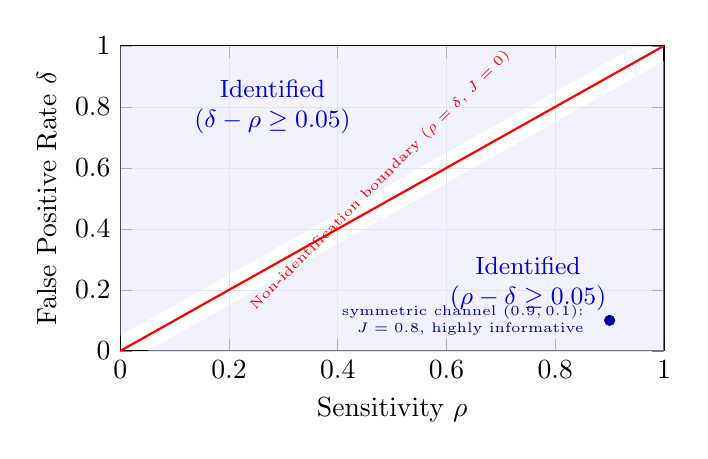
\begin{tikzpicture}
\begin{axis}[
    width=0.7\textwidth,
    height=0.45\textwidth,
    xlabel={Sensitivity $\rho$},
    ylabel={False Positive Rate $\delta$},
    xmin=0, xmax=1,
    ymin=0, ymax=1,
    grid=both,
    grid style={line width=.1pt, draw=gray!10},
    major grid style={line width=.2pt, draw=gray!20},
]
% Identified regions: |rho - delta| >= 0.05 on either side of the diagonal
\fill[blue!10, opacity=0.5] (axis cs: 0, 0.05) -- (axis cs: 0.95, 1) -- (axis cs: 0, 1) -- cycle; % %%NEEDS_HUMAN_MATH_REVIEW%%
\fill[blue!10, opacity=0.5] (axis cs: 0.05, 0) -- (axis cs: 1, 0.95) -- (axis cs: 1, 0) -- cycle; % %%NEEDS_HUMAN_MATH_REVIEW%%

% Diagonal line (the only non-identification boundary)
\addplot[thick, red, domain=0:1] {x};
\node[anchor=south, rotate=45, text=red, font=\tiny] at (axis cs: 0.5, 0.52) {Non-identification boundary ($\rho = \delta$, $J = 0$)}; % %%NEEDS_HUMAN_MATH_REVIEW%%

\node[text=blue!85!black, font=\small, align=center] at (axis cs: 0.28, 0.8) {Identified\\($\delta - \rho \ge 0.05$)};
\node[text=blue!85!black, font=\small, align=center] at (axis cs: 0.75, 0.22) {Identified\\($\rho - \delta \ge 0.05$)};

% Example: the symmetric channel rho = 1 - delta is NOT a boundary
\addplot[only marks, mark=*, mark size=1.8pt, color=blue!60!black] coordinates {(0.9, 0.1)}; % %%NEEDS_HUMAN_MATH_REVIEW%%
\node[anchor=east, text=blue!60!black, font=\tiny, align=right] at (axis cs: 0.87, 0.1) {symmetric channel $(0.9, 0.1)$:\\$J = 0.8$, highly informative};

\end{axis}
\end{tikzpicture}
\caption{Parameter space of source channels. The only non-identification boundary is the diagonal $\rho = \delta$, where the Youden index $J = |\rho - \delta|$ vanishes; Gate FG2 excludes the band $|\rho - \delta| < 0.05$ around it. The anti-diagonal $\rho = 1 - \delta$, marked as a ``label flip boundary'' in an earlier draft, is \emph{not} a singular set: the symmetric channel $(0.9, 0.1)$ lies on it and is among the most informative channels. Both off-diagonal regions ($\rho - \delta \ge 0.05$ and $\delta - \rho \ge 0.05$) are rank-identifiable up to the label swap; the production implementation orients the activity class by enforcing $\rho_s > \delta_s$, so anti-informative channels ($\delta_s > \rho_s$) are either relabeled or excluded from headline interpretation.} % %%NEEDS_HUMAN_MATH_REVIEW%%
\label{fig:parameter_space}
\end{figure}

---

\section{Theorem $B'$ --- Bayes Error \& Information Scaling under $N \cdot I^2$}

\subsection{Setting}
We consider a single binary channel $Y \in \{0, 1\}$ measuring a latent state $A \in \{0, 1\}$. We seek the relationship between the channel informativeness $I$ and the minimum classification error rate, and the scaling of the Fisher information for the prevalence parameter $\phi$. The scope of this section is fixed by three explicit assumptions: % %%NEEDS_HUMAN_MATH_REVIEW%%
\begin{itemize}
    \item[(B1)] \textbf{Known channel.} The channel parameters $(\rho, \delta)$ are treated as known. In the engine they are not known a priori: they are identified by the $S \ge 3$ source layer of Theorem $A'$ and estimated jointly with $\phi$. Theorem $B'.2$ is therefore a statement about the \emph{conditional} Fisher information given $(\rho, \delta)$ --- an upper bound on the information available when $(\rho, \delta)$ must themselves be estimated (see the remark following the proof). % %%NEEDS_HUMAN_MATH_REVIEW%%
    \item[(B2)] \textbf{Independent replicate units.} The $N$ observations are labels on $N$ distinct units, each carrying an independent fresh draw $A_u \sim \mathrm{Bernoulli}(\phi)$, as in (A1). $N$ does \emph{not} count repeated measurements of one unit, nor serially dependent observations; both failure modes are quantified in the remark below and in the dependent-sample correction of Section 7.2. % %%NEEDS_HUMAN_MATH_REVIEW%%
    \item[(B3)] \textbf{Label noise as the only noise source.} The marginal variance $p(1-p)$ reflects channel noise and prevalence variation only. Coder noise, observability variation, and selection effects --- all present in the production likelihood --- further reduce the usable information, so the formulas of this section are upper bounds in the production setting. % %%NEEDS_HUMAN_MATH_REVIEW%%
\end{itemize}

\subsection{Formal Statement}
Define the channel \textbf{informativeness} $I$ as:
\[
I = |\rho - \delta| \in [0, 1]
\]

\begin{theorem}[Bayes Error \& Information Scaling]
Under the stated binary channel model and (B1)--(B3):
\begin{enumerate}
    \item (Theorem $B'.1$): Under equal prior odds ($P(A=1) = 0.5$), the minimum classification error $\varepsilon^\star$ for recovering $A$ from a single observation $Y$ is:
    \[
    \varepsilon^\star = \frac{1}{2}(1 - I)
    \]
    \item (Theorem $B'.2$): The conditional Fisher information $I_F(\phi)$ about the latent activity prevalence $\phi$, given known $(\rho, \delta)$, from $N$ independent replicate units is: % %%NEEDS_HUMAN_MATH_REVIEW%%
    \[
    I_F(\phi) = N \frac{I^2}{p(1-p)}
    \]
    where $p = P(Y=1) = \delta + I\phi$ (assuming $\rho > \delta$).
\end{enumerate}
\end{theorem}

\subsection{Step-by-Step Proof}

\subsubsection{Proof of Theorem $B'.1$}
\begin{proof}
Let $g(Y) \in \{0, 1\}$ be any decision rule (classifier) mapping the observed label $Y$ to an estimate of the latent state $A$. The probability of classification error is:
\[
P(\text{Error}) = P(g(Y) \neq A)
\]
Under equal priors ($P(A=1) = P(A=0) = 0.5$), the minimum error probability is achieved by the MAP (Maximum A Posteriori) decision rule, which is the Bayes classifier. The Bayes error $\varepsilon^\star$ is given by:
\[
\varepsilon^\star = \frac{1}{2} \left( 1 - \text{TV}(P_{Y \mid A=1}, P_{Y \mid A=0}) \right)
\]
where $\text{TV}$ is the Total Variation distance between the two class-conditional probability laws of $Y$. Since $Y$ is a binary random variable, $P_{Y \mid A=1} \sim \text{Bernoulli}(\rho)$ and $P_{Y \mid A=0} \sim \text{Bernoulli}(\delta)$. 

We compute the Total Variation distance:
\begin{align*}
    \text{TV}(P_{Y \mid A=1}, P_{Y \mid A=0}) &= \frac{1}{2} \sum_{y \in \{0, 1\}} |P(Y=y \mid A=1) - P(Y=y \mid A=0)| \\
    &= \frac{1}{2} \Big( |P(Y=1 \mid A=1) - P(Y=1 \mid A=0)| \\
    &\quad\quad + |P(Y=0 \mid A=1) - P(Y=0 \mid A=0)| \Big) \\
    &= \frac{1}{2} \left( |\rho - \delta| + |(1 - \rho) - (1 - \delta)| \right) \\
    &= \frac{1}{2} \left( |\rho - \delta| + |\delta - \rho| \right) \\
    &= |\rho - \delta| = I
\end{align*}
Substituting $\text{TV} = I$ into the Bayes error equation:
\[
\varepsilon^\star = \frac{1}{2}(1 - I)
\]
Any classifier trying to predict $A$ using only $Y$ must suffer an error rate of at least $\frac{1}{2}(1 - I)$.
\end{proof}

\begin{remark}[Unequal priors and the usefulness window]
Theorem $B'.1$ is stated at the balanced operating point $P(A{=}1) = 0.5$, where it isolates channel quality from prior imbalance. For a general prior $\phi$, the Bayes error is
\[
\varepsilon^\star(\phi) = \frac{1}{2}\Big(1 - \sum_{y \in \{0,1\}} \big| \phi\, P(Y{=}y \mid A{=}1) - (1-\phi)\, P(Y{=}y \mid A{=}0) \big| \Big), % %%NEEDS_HUMAN_MATH_REVIEW%%
\]
which reduces to $\frac{1}{2}(1 - I)$ at $\phi = 0.5$. Under strong imbalance the MAP rule ignores the observation entirely: for $\rho > \delta$, the single observation $Y$ affects the decision if and only if the prior odds lie in the window % %%NEEDS_HUMAN_MATH_REVIEW%%
\[
\frac{\delta}{\rho} \;\le\; \frac{\phi}{1 - \phi} \;\le\; \frac{1 - \delta}{1 - \rho}. % %%NEEDS_HUMAN_MATH_REVIEW%%
\]
Outside this window, $\varepsilon^\star(\phi) = \min(\phi, 1 - \phi)$ is achieved by the constant classifier and the channel contributes nothing --- the single-observation form of prior domination. The engine therefore uses the balanced-prior quantity $\frac{1}{2}(1 - I)$ as a \emph{channel-quality benchmark}, not as the operational error rate of any production decision. % %%NEEDS_HUMAN_MATH_REVIEW%%
\end{remark}

\subsubsection{Proof of Theorem $B'.2$}
\begin{proof}
Let $Y_1, \dots, Y_N$ be $N$ conditionally independent binary observations from a channel with parameters $\rho, \delta$ and informativeness $I = |\rho - \delta|$. Let $Y \sim \text{Bernoulli}(p)$ be a single binary observation. Assuming without loss of generality that $\rho > \delta$, the success probability is:
\[
p = \delta + \phi(\rho - \delta) = \delta + I\phi
\]
The probability mass function of $Y$ is:
\[
f(y \mid \phi) = p^y (1 - p)^{1 - y}
\]
Taking the natural logarithm:
\[
\ln f(y \mid \phi) = y \ln(p) + (1 - y) \ln(1 - p)
\]
We compute the score function by taking the partial derivative with respect to $\phi$:
\[
\frac{\partial}{\partial \phi} \ln f(y \mid \phi) = y \frac{1}{p} \frac{\partial p}{\partial \phi} - (1 - y) \frac{1}{1 - p} \frac{\partial p}{\partial \phi}
\]
Since $\frac{\partial p}{\partial \phi} = \frac{\partial}{\partial \phi} (\delta + I\phi) = I$:
\[
\frac{\partial}{\partial \phi} \ln f(y \mid \phi) = I \left( \frac{y}{p} - \frac{1 - y}{1 - p} \right) = I \frac{y - p}{p(1 - p)}
\]
The Fisher information of a single observation is the variance of the score function:
\begin{align*}
    I_{F, 1}(\phi) &= E\left[ \left( \frac{\partial}{\partial \phi} \ln f(Y \mid \phi) \right)^2 \right] \\
    &= E\left[ \frac{I^2 (Y - p)^2}{p^2 (1 - p)^2} \right] \\
    &= \frac{I^2}{p^2 (1 - p)^2} E[(Y - p)^2]
\end{align*}
Since $Y \sim \text{Bernoulli}(p)$, its variance is $E[(Y - p)^2] = \text{Var}(Y) = p(1-p)$. Substituting this:
\[
I_{F, 1}(\phi) = \frac{I^2}{p^2 (1 - p)^2} p(1 - p) = \frac{I^2}{p(1 - p)}
\]
By the additivity of Fisher information for $N$ independent units (B2), the total Fisher information is:
\[
I_F(\phi) = N \cdot I_{F, 1}(\phi) = N \frac{I^2}{p(1 - p)}
\]
This completes the proof.
\end{proof}

\begin{remark}[What Theorem $B'.2$ does and does not assert]
\begin{enumerate}
    \item \textbf{Conditional information only.} The formula conditions on known $(\rho, \delta)$ per (B1). When $(\rho, \delta)$ are estimated jointly with $\phi$, the efficient information for $\phi$ is the Schur complement
\[
I_{\phi\phi} - I_{\phi\eta}\, I_{\eta\eta}^{-1}\, I_{\eta\phi} \;\le\; I_{\phi\phi}, \qquad \eta = (\rho, \delta), % %%NEEDS_HUMAN_MATH_REVIEW%%
\]
which is strictly smaller whenever the cross-information is nonzero. Indeed, from a \emph{single} channel the triple $(\phi, \rho, \delta)$ is not identifiable at all --- the marginal law carries a single degree of freedom, $p = \delta + I\phi$. The conditional formula is meaningful only because the $S \ge 3$ source layer of Theorem $A'$ identifies $(\rho, \delta)$. % %%NEEDS_HUMAN_MATH_REVIEW%%
    \item \textbf{$N$ counts independent units.} If the $N$ observations were repeated measurements of a \emph{single} unit (one draw of $A$), the information about $\phi$ would saturate: even perfect recovery of that unit's $A$ yields the information of one clean $\mathrm{Bernoulli}(\phi)$ observation, $1/(\phi(1-\phi))$, no matter how many labels are taken. Linear-in-$N$ scaling requires a fresh latent draw per unit, as stated in (B2). % %%NEEDS_HUMAN_MATH_REVIEW%%
    \item \textbf{Exact clean-label equivalent.} Equating the noisy-label variance bound $p(1-p)/(N I^2)$ with the clean-label variance $\phi(1-\phi)/N_{\mathrm{eq}}$ gives the exact equivalent clean sample size $N_{\mathrm{eq}} = N I^2\, \phi(1-\phi)/(p(1-p))$. The engine's working quantity $N \cdot I^2$ is this expression with the factor $\phi(1-\phi)/(p(1-p))$ set to one; that factor can fall on either side of one, so $N \cdot I^2$ is an order-of-magnitude proxy, not a bound in a fixed direction, and the floor of Gate FG3 below is calibrated to it as such. % %%NEEDS_HUMAN_MATH_REVIEW%%
\end{enumerate}
\end{remark}

\subsection{The Quadratic Collapse ($I \to 0$)}
The denominator $p(1 - p)$ represents the variance of the observed data and is bounded by $0.25$ (achieved when $p = 0.5$). Thus, we establish the inequality:
\begin{equation}\label{eq:scaling_bound}
I_F(\phi) \ge 4 N \cdot I^2
\end{equation}
with equality if and only if $p = 1/2$; for $p \neq 1/2$ the inequality is strict. The quantity $4NI^2$ is therefore a \emph{lower bound} on the Fisher information, not the Fisher information itself --- Figure~\ref{fig:information_diagnostics} plots this bound. % %%NEEDS_HUMAN_MATH_REVIEW%%
By the Cramer-Rao bound, the variance of any unbiased estimator $\hat{\phi}$ is bounded by the reciprocal of the Fisher information:
\[
\text{Var}(\hat{\phi}) \ge \frac{1}{I_F(\phi)} = \frac{p(1-p)}{N \cdot I^2}
\]
To maintain a constant estimation precision $\sigma^2 = \text{Var}(\hat{\phi})$, the required sample size scales as:
\[
N \propto \frac{1}{I^2}
\]
If a source's informativeness drops by a factor of 10, you need \textbf{100 times more data} to achieve the same confidence.

\subsection{Operational Diagnostic}
\begin{itemize}
    \item \textbf{Kernel Location:} \href{file:///Users/arbenlila/development/david/canonical/david/theorems/B_prime.py}{\texttt{david/theorems/B\_prime.py}}
    \item \textbf{Gate Rule (FG3), two co-registered conditions} --- checked at the cell level; \emph{both} must hold (constants in \texttt{david/config.py}): % %%NEEDS_HUMAN_MATH_REVIEW%%
    \begin{enumerate}
        \item \textbf{Informativeness floor:} the lower endpoint of the central 95\% credible interval of $I(O)$ (the 2.5\% posterior quantile) must satisfy
        \[
        I_{\text{lower 95\%}} \ge \texttt{INFORMATIVENESS\_FLOOR\_LOWER\_95} = 0.10 % %%NEEDS_HUMAN_MATH_REVIEW%%
        \]
        \item \textbf{Information floor:} the effective information must satisfy
        \[
        N_{\mathrm{eff}} \cdot I^2 \ge \texttt{N\_EFF\_I2\_FLOOR} = 3.0 % %%NEEDS_HUMAN_MATH_REVIEW%%
        \]
        where $I$ is the posterior median informativeness and $N_{\mathrm{eff}}$ is the replicate count, dependence-adjusted per Section 7.2 when units are serially correlated. % %%NEEDS_HUMAN_MATH_REVIEW%%
    \end{enumerate}
    If either condition fails, the cell is routed as \texttt{prior\_dominated} and represented as an uninformative prior interval.
\end{itemize}

\begin{remark}[Why the information floor is $3.0$]
By the Cram\'er--Rao bound and Theorem $B'.2$, $\mathrm{Var}(\hat{\phi}) \ge p(1-p) / (N_{\mathrm{eff}} I^2)$, and $p(1-p) \le 1/4$, so Under the efficient-asymptotic approximation, $N_{\mathrm{eff}} I^2 \ge 3$ makes the Cram\'er--Rao inverse-information scale no larger than $1/12$, the variance of a $\mathrm{Uniform}(0,1)$ prior at the worst operating point $p = 1/2$. The Cram\'er--Rao bound is a \emph{lower} bound on estimator variance, so this says: an efficient asymptotic estimator \emph{could} beat the flat-prior variance, but there is no guarantee that any finite-sample estimator achieves it. Below the floor, even the Cram\'er--Rao benchmark cannot match the flat-prior variance: at worst-case $p \approx 1/2$ no unbiased estimator can improve on knowing nothing, and the cell is prior-dominated. % %%NEEDS_HUMAN_MATH_REVIEW%% This calibration argument fixes the order of the constant, not its third digit; the specific value $3.0$ is pre-registered (\texttt{N\_EFF\_I2\_FLOOR}). The floor also closes a gap left by the informativeness floor alone: a cell with $I = 0.11$ and $N = 5$ replicates passes condition 1 marginally yet has $N I^2 \approx 0.06 \ll 3$, and is correctly rejected by condition 2. % %%NEEDS_HUMAN_MATH_REVIEW%%
\end{remark}

\begin{figure}[htbp]
\centering
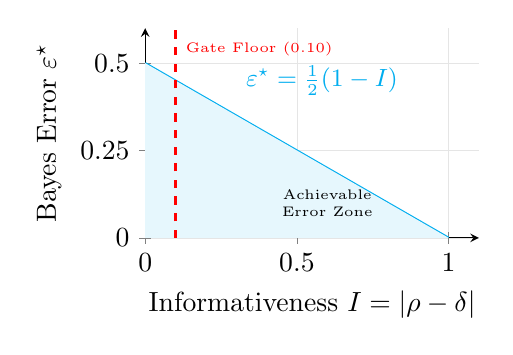
\begin{tikzpicture}
\begin{axis}[
    width=0.48\textwidth,
    height=0.35\textwidth,
    axis lines=left,
    xlabel={Informativeness $I = |\rho - \delta|$},
    ylabel={Bayes Error $\varepsilon^\star$},
    xmin=0, xmax=1.1,
    ymin=0, ymax=0.6,
    xtick={0, 0.5, 1},
    ytick={0, 0.25, 0.5},
    grid=both,
    grid style={line width=.1pt, draw=gray!10},
    major grid style={line width=.2pt, draw=gray!20},
]
\addplot[thick, cyan, domain=0:1] {0.5*(1 - x)};
\addplot[fill=cyan!10, draw=none, domain=0:1] {0.5*(1 - x)} \closedcycle;
\node[anchor=south west, text=cyan, font=\small] at (axis cs: 0.3, 0.38) {$\varepsilon^\star = \frac{1}{2}(1 - I)$};
\draw[dashed, red, thick] (axis cs: 0.1, 0) -- (axis cs: 0.1, 0.6) node[pos=0.9, right, font=\tiny] {Gate Floor ($0.10$)};
\node[align=center, font=\tiny] at (axis cs: 0.6, 0.1) {Achievable\\Error Zone};
\end{axis}
\end{tikzpicture}
\hfill
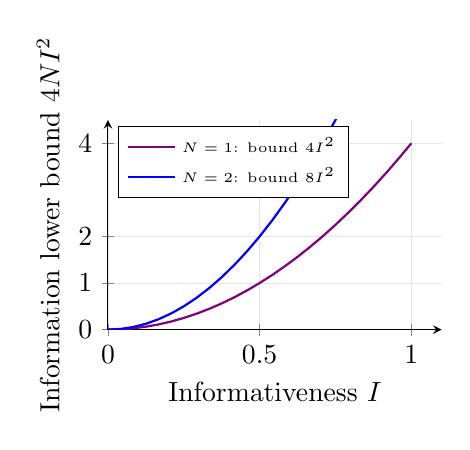
\begin{tikzpicture}
\begin{axis}[
    width=0.48\textwidth,
    height=0.35\textwidth,
    axis lines=left,
    xlabel={Informativeness $I$},
    ylabel={Information lower bound $4NI^2$},
    xmin=0, xmax=1.1,
    ymin=0, ymax=4.5,
    xtick={0, 0.5, 1},
    ytick={0, 1, 2, 4},
    grid=both,
    grid style={line width=.1pt, draw=gray!10},
    major grid style={line width=.2pt, draw=gray!20},
    legend pos=north west,
    legend style={font=\tiny},
]
\addplot[thick, violet, domain=0:1] {4*x^2};
\addlegendentry{$N = 1$: bound $4 I^2$}
\addplot[thick, blue, domain=0:1] {8*x^2};
\addlegendentry{$N = 2$: bound $8 I^2$}
\node[anchor=west, align=left, font=\tiny, text=violet] at (axis cs: 0.1, 3.2) {Quadratic Collapse\\as $I \to 0$};
\end{axis}
\end{tikzpicture}
\caption{Bayes classification error $\varepsilon^\star$ (left) and the Fisher-information \emph{lower bound} $4NI^2 \le I_F(\phi)$ of Eq.~\eqref{eq:scaling_bound} (right), plotted against channel informativeness $I$. The bound is tight only at $p = 1/2$; the true $I_F(\phi)$ lies on or above the plotted curves. The red dashed line denotes the $I \ge 0.10$ information gate.} % %%NEEDS_HUMAN_MATH_REVIEW%%
\label{fig:information_diagnostics}
\end{figure}

---

\section{Theorem $C$ --- Dependency-Robust Posterior Expected FDP Control}

\subsection{Setting and Scope of the Guarantee}
In multi-cell forecasting we make multiple binary flagging decisions and wish to control the False Discovery Proportion (FDP). Forecast cells are strongly dependent --- spatially, temporally, and across horizons within a stratum --- so $p$-value-based procedures such as Benjamini--Hochberg are not applicable off the shelf: their guarantees require independence or positive regression dependency (PRDS), and the engine produces no per-cell $p$-values in the first place. We therefore control the \emph{posterior expected} FDP. Two scope qualifications are part of the claim itself: % %%NEEDS_HUMAN_MATH_REVIEW%%
\begin{enumerate}
    \item The guarantee is an expectation under the joint posterior of the latent activity vector given the data. It is \emph{not} distribution-free in the frequentist sense, and it is not the frequentist FDR $E_{\text{sampling}}[\mathrm{FDP}]$, which averages over hypothetical repeated data sets; the conditioning is on the one observed data set. % %%NEEDS_HUMAN_MATH_REVIEW%%
    \item The guarantee is conditional on the validity of the posterior: if the model's marginal posterior probabilities $p_i$ are miscalibrated, the bound is a statement about the model's internal beliefs, not about reality. Posterior validity is supported operationally --- simulation-based calibration (Section 8) and the gold-label coder calibration --- and the conditionality is carried in the theorem's name rather than hidden. % %%NEEDS_HUMAN_MATH_REVIEW%%
\end{enumerate}

\subsection{Formal Statement}
Let $p_i = P(A_i = 1 \mid \text{data})$ be the marginal posterior probability of activity for cell $i \in \{1, \dots, M\}$. Let $d_i \in \{0, 1\}$ represent the decision to flag cell $i$ as active ($d_i=1$) or inactive ($d_i=0$).

Sort the cells by their posterior probabilities in descending order:
\[
p_{(1)} \ge p_{(2)} \ge \dots \ge p_{(M)}
\]
Define the decision rule $d_{(j)} = 1$ for $j \le m^\star$ and $d_{(j)} = 0$ for $j > m^\star$, where:
\begin{equation}\label{eq:fdp_cutoff}
m^\star = \max\Big\{ m : \frac{1}{m}\sum_{j=1}^{m}\big(1 - p_{(j)}\big) \le q \Big\}, \qquad \max \emptyset := 0. % %%NEEDS_HUMAN_MATH_REVIEW%%
\end{equation}
The rule is well defined: since $1 - p_{(j)}$ is nondecreasing in $j$, the running average $\frac{1}{m}\sum_{j \le m}(1 - p_{(j)})$ is nondecreasing in $m$, so the feasible set is the interval $\{1, \dots, m^\star\}$ (or empty, in which case no cell is flagged). % %%NEEDS_HUMAN_MATH_REVIEW%%

\begin{theorem}[Posterior Expected FDP Control under Arbitrary Latent Dependence]
The decision rule $m^\star$ guarantees that the posterior expected False Discovery Proportion is bounded by $q$:
\[
E[\mathrm{FDP} \mid \mathcal{D}] \le q,
\]
where the expectation is taken under the joint posterior law of $(A_1, \dots, A_M)$ given the observed data $\mathcal{D}$. The bound holds for \emph{every} joint dependence structure among $A_1, \dots, A_M$ consistent with the marginal posteriors $p_i$, and is conditional on those marginal posterior probabilities being valid. % %%NEEDS_HUMAN_MATH_REVIEW%%
\end{theorem}

\subsection{Step-by-Step Proof}
\begin{proof}
Let the total number of flagged cells (discoveries) be $D = \sum_{i=1}^M d_i$. Let $V$ be the number of falsely flagged cells (false discoveries):
\[
V = \sum_{i=1}^M d_i (1 - A_i)
\]
where $A_i \in \{0, 1\}$ is the true latent activity. The False Discovery Proportion (FDP) is the random variable defined as:
\[
\text{FDP} = \frac{V}{\max(1, D)} = \frac{\sum_{i=1}^M d_i (1 - A_i)}{\max(1, \sum_{i=1}^M d_i)}
\]
Let $\mathcal{D}$ denote the observed data. We evaluate the expectation of this random variable over the joint posterior distribution of $\mathbf{A} = (A_1, \dots, A_M)^T$ conditioned on the observed data $\mathcal{D}$. 

Since the decision vector $\mathbf{d}$ is a deterministic function of the observed data $\mathcal{D}$ (as it is computed entirely from the marginal posterior probabilities $p_i = P(A_i = 1 \mid \mathcal{D})$), both the indicators $d_i$ and the denominator $D = \max(1, \sum d_i)$ are $\sigma(\mathcal{D})$-measurable. Consequently, they are constant under the conditional expectation $E[\,\cdot \mid \mathcal{D}]$.

By the linearity of conditional expectation, we can pull the denominator and the decision indicators out of the expectation:
\begin{align}
    E[\text{FDP} \mid \mathcal{D}] &= E\left[ \frac{\sum_{i=1}^M d_i (1 - A_i)}{\max(1, D)} \;\middle|\; \mathcal{D} \right] \nonumber \\
    &= \frac{1}{\max(1, D)} \sum_{i=1}^M d_i E[1 - A_i \mid \mathcal{D}] \label{eq:linearity}
\end{align}
We evaluate the conditional expectation of the term $1 - A_i$:
\[
E[1 - A_i \mid \mathcal{D}] = 1 - E[A_i \mid \mathcal{D}] = 1 - P(A_i = 1 \mid \mathcal{D}) = 1 - p_i
\]
Substituting this back into Equation~\eqref{eq:linearity}:
\begin{equation}\label{eq:fdp_exp_simplified}
E[\text{FDP} \mid \mathcal{D}] = \frac{1}{\max(1, D)} \sum_{i=1}^M d_i (1 - p_i)
\end{equation}
Under our decision rule, we flag the top $m$ sorted cells. Thus, $d_{(j)} = 1$ for $j \le m$, and $d_{(j)} = 0$ for $j > m$, which implies the number of discoveries is $D = m$.
If $m = 0$, then $D = 0$, and by definition $\text{FDP} = 0$, which trivially satisfies $0 \le q$.
For any $m \ge 1$, we substitute the decision rule into Equation~\eqref{eq:fdp_exp_simplified}:
\[
E[\text{FDP} \mid \mathcal{D}] = \frac{1}{m} \sum_{j=1}^m (1 - p_{(j)})
\]
By choosing $m^\star$ as the largest integer $m$ satisfying:
\[
\frac{1}{m} \sum_{j=1}^m (1 - p_{(j)}) \le q
\]
we guarantee that:
\[
E[\text{FDP} \mid \mathcal{D}] \le q
\]
Because the proof relies only on the linearity of conditional expectation, it does not require independence of the variables $A_i$: the posterior \emph{expectation} of the FDP is a function of the marginal posteriors $p_i$ alone, whatever the joint dependence (Newton et al., 2004; M\"uller et al., 2004). Two caveats delimit the result. First, this is robustness to \emph{latent} dependence, not distribution-freeness: every $p_i$ is computed under the model, so the guarantee is conditional on the model's posterior being valid --- a condition that is tested (SBC, coder calibration), not assumed away. Second, only the expectation of the FDP is controlled; its dispersion under dependence is the subject of the exceedance challenge and defense in Section 7. % %%NEEDS_HUMAN_MATH_REVIEW%%
\end{proof}

\subsection{Operational Diagnostic}
\begin{itemize}
    \item \textbf{Kernel Location:} \href{file:///Users/arbenlila/development/david/canonical/david/theorems/C_renamed.py}{\texttt{david/theorems/C\_renamed.py}}
    \item \textbf{Routing Logic:} Unlike Theorems $A'$ and $B'$, Theorem $C$ does not block the MCMC fit. It computes the threshold probability $t^\star(q) = p_{(m^\star)}$ (defined when $m^\star \ge 1$; if $m^\star = 0$, no cell is flagged and the control is vacuously satisfied) and dynamically tightens the set of flagged active cells under the pre-registered default $q = 0.10$ (\texttt{POSTERIOR\_FDP\_DEFAULT\_Q}). Both this expectation control and the exceedance control of Section 7 are conditional on posterior validity in the sense of the theorem statement. % %%NEEDS_HUMAN_MATH_REVIEW%%
\end{itemize}

---

\section{Theorem $D$-forecast --- Ergodic Convergence and the Horizon Diagnostic $h^\star$}

\subsection{Setting}
Let the latent regimes follow a discrete-time (monthly) Hidden Semi-Markov Model (HSMM) with $L$ states. The transition behavior is governed by: (i) a transition matrix $\Pi \in \mathbb{R}^{L \times L}$ of the embedded chain, with zero diagonal ($\pi_{ii} = 0$, enforcing state changes); and (ii) dwell-time laws $f_r$ on $\{1, 2, \dots\}$ with finite means $\mu_r$, for each state $r \in \{1, \dots, L\}$ (the implementation uses shifted-Poisson dwell). The minimal Markov state of the system is the \emph{pair} $(Z_t, a_t)$, where $a_t$ is the elapsed dwell age in the current regime; $Z_t$ alone is not Markov unless the dwell laws are geometric. We seek an operational diagnostic horizon $h^\star$ beyond which a conditional forecast is dominated by the prior --- a diagnostic threshold, not an exact validity boundary. % %%NEEDS_HUMAN_MATH_REVIEW%%

\begin{remark}[Why the dwell age cannot be dropped: a minimal example]
Take $L = 2$ states with deterministic dwell $D \equiv 3$ months and forced alternation ($\pi_{12} = \pi_{21} = 1$). Then % %%NEEDS_HUMAN_MATH_REVIEW%%
\[
P(Z_{t+1} = 1 \mid Z_t = 1, a_t = 0) = 1, \qquad P(Z_{t+1} = 1 \mid Z_t = 1, a_t = 2) = 0, % %%NEEDS_HUMAN_MATH_REVIEW%%
\]
since a regime aged $0$ months has two months remaining while a regime aged $2$ ends now. Averaging over the stationary age distribution (uniform on $\{0, 1, 2\}$) gives $P(Z_{t+1} = 1 \mid Z_t = 1) = 2/3$: the age-free quantity is a $2/3$--$1/3$ blur of two \emph{deterministic} futures, and no one-step kernel on $Z$ alone reproduces the process. For geometric dwell the conditional probabilities coincide for every age (memorylessness) --- precisely the special case in which the HSMM degenerates to a Markov chain and conditioning on $Z_t$ alone is sufficient. % %%NEEDS_HUMAN_MATH_REVIEW%%
\end{remark}

\subsection{Formal Statement}
Let the embedded Markov chain of state changes have a unique stationary eigenvector $\nu$ satisfying $\nu \Pi = \nu$ and $\sum \nu_r = 1$. The time-weighted stationary marginal probability $\pi_\infty \in \mathbb{R}^L$ of being in regime $r$ is:
\begin{equation}\label{eq:stationary_marginal}
\pi_\infty[r] = \frac{\nu[r]\,\mu[r]}{\sum_{j=1}^{L} \nu[j]\,\mu[j]}
\end{equation}
Per the remark above, the forecast distribution must carry the dwell age. We define % %%NEEDS_HUMAN_MATH_REVIEW%%
\[
\text{forecast}_h = P(Z_{t+h} \mid Z_t, a_t, \text{data}), % %%NEEDS_HUMAN_MATH_REVIEW%%
\]
or, when the age at the forecast origin is uncertain (as it is at a right-censored series end), the posterior age mixture $\sum_{a} P(Z_{t+h} \mid Z_t, a, \text{data})\, P(a_t = a \mid \text{data})$. The \textbf{prior-drift share} is defined as: % %%NEEDS_HUMAN_MATH_REVIEW%%
\begin{equation}\label{eq:prior_drift}
\text{drift}(h) = 1 - \frac{\text{TV}(\text{forecast}_h,\ \pi_\infty)}{\text{TV}(\text{forecast}_h,\ \pi_\infty) + \text{TV}(\text{forecast}_h,\ z_t)}
\end{equation}
where $z_t[r] = \mathbb{I}(Z_t = r)$ is the Kronecker delta distribution for the \emph{known-state} case (the theoretical benchmark). In the operational hidden-state setting the current regime is not observed; $z_t$ should be replaced by the posterior state distribution $\zeta_t[r] = P(Z_t = r \mid D_{1:t})$, computed by the HSMM forward filter, and the prior-drift share should correspondingly be evaluated at $\zeta_t$ rather than at a point mass. The first claim of Theorem $D$ (convergence to $\pi_\infty$) holds under both the conditional and the posterior-averaged forecast; the Kronecker form is retained in the theorem statement for clarity. % %%NEEDS_HUMAN_MATH_REVIEW%%

\begin{theorem}[Ergodic Horizon Bound]
Assume: % %%NEEDS_HUMAN_MATH_REVIEW%%
\begin{itemize}
    \item[(D1)] the embedded chain $\Pi$ is irreducible (aperiodicity of $\Pi$ is \emph{not} assumed --- see the note below); % %%NEEDS_HUMAN_MATH_REVIEW%%
    \item[(D2)] each dwell law $f_r$ has finite mean and aperiodic lattice support: $\gcd\{d : f_r(d) > 0\} = 1$ (satisfied by the shifted-Poisson dwell, whose support is all of $\{1, 2, \dots\}$). % %%NEEDS_HUMAN_MATH_REVIEW%%
\end{itemize}
Then, for every initial regime $i$ and elapsed age $a$:
\begin{enumerate}
    \item The conditional forecast converges to the time-weighted stationary distribution:
    \[
    \lim_{h \to \infty} P(Z_{t+h} = r \mid Z_t = i,\, a_t = a) = \pi_\infty[r], % %%NEEDS_HUMAN_MATH_REVIEW%%
    \]
    and hence the same limit holds for the age-mixed forecast.
    \item The prior-drift share converges to 1:
    \[
    \lim_{h \to \infty} \text{drift}(h) = 1
    \]
\end{enumerate}
\end{theorem}

\noindent\textbf{Note on the hypotheses.} An earlier draft assumed an ``irreducible and aperiodic embedded chain.'' That hypothesis is unsatisfiable in this model class for $L = 2$: with zero diagonal, the embedded chain necessarily alternates and is $2$-periodic. Aperiodicity of the \emph{embedded} chain is neither available nor needed; what drives time-domain mixing in a semi-Markov process is the lattice aperiodicity of the dwell laws (D2), which makes the return-time distributions to each state aperiodic even when the embedded chain is periodic. % %%NEEDS_HUMAN_MATH_REVIEW%%

\subsection{Step-by-Step Proof}
\begin{proof}
Let $T_n$ denote the time of the $n$-th regime transition. The sequence of states $Z_{T_n}$ forms the embedded Markov chain. Since $\Pi$ is finite and irreducible (D1), it has a unique stationary distribution $\nu$ satisfying $\nu \Pi = \nu$ with $\nu > 0$ (Perron--Frobenius), and the embedded chain is positive recurrent. We emphasize that no convergence of the embedded chain's marginals is claimed or needed --- the embedded chain may be periodic (it always is for $L = 2$); only its stationary distribution $\nu$ and recurrence structure enter the argument. % %%NEEDS_HUMAN_MATH_REVIEW%%

The process $Z_t$ is a discrete-time semi-Markov process in which the dwell time in state $r$ has law $f_r$ and mean $\mu[r]$. To find the limiting time-average occupation of $Z_t$, we apply the \textbf{Renewal Reward Theorem}.
Let $N_r(t)$ be the number of visits to state $r$ by time $t$. The long-run proportion of time spent in state $r$ is:
\[
P_\infty(r) = \lim_{t \to \infty} \frac{1}{t} \sum_{s=1}^{t} \mathbb{I}(Z_s = r) \quad \text{a.s.} % %%NEEDS_HUMAN_MATH_REVIEW%%
\]
We define a cycle as the time between successive entries into a reference state, say state 1. The expected cycle length is the sum of the expected time spent in each state during a cycle:
\[
E[\text{Cycle}] = \sum_{j=1}^L E[\text{Visits to } j \text{ per cycle}] \cdot E[D_j]
\]
From renewal theory and embedded chain dynamics, the expected number of visits to state $j$ between consecutive visits to state 1 is $\frac{\nu[j]}{\nu[1]}$. Since the expected dwell time is $E[D_j] = \mu[j]$:
\[
E[\text{Cycle}] = \sum_{j=1}^L \frac{\nu[j]}{\nu[1]} \mu[j] = \frac{1}{\nu[1]} \sum_{j=1}^L \nu[j] \mu[j]
\]
The expected time spent in state $r$ during a single cycle is:
\[
E[\text{Time in state } r] = \frac{\nu[r]}{\nu[1]} \mu[r]
\]
By the Renewal Reward Theorem, the stationary probability is:
\[
\pi_\infty[r] = \frac{E[\text{Time in state } r]}{E[\text{Cycle}]} = \frac{\frac{\nu[r]}{\nu[1]} \mu[r]}{\frac{1}{\nu[1]} \sum_{j=1}^L \nu[j] \mu[j]} = \frac{\nu[r] \mu[r]}{\sum_{j=1}^L \nu[j] \mu[j]}
\]
The renewal-reward argument gives the time-\emph{average}; the pointwise limit requires a renewal theorem, and here the lattice structure matters. The dwell laws are supported on the integer (monthly) lattice, so the classical Key Renewal Theorem for non-lattice distributions does \emph{not} apply; the correct tool is the lattice (discrete-time) Markov renewal theorem, the multi-state extension of the Erd\H{o}s--Feller--Pollard renewal theorem. Under (D1)--(D2), the distribution of the return time to any fixed state has period $\gcd = 1$: return times are sums of dwell draws along recurrence cycles, and since each $f_r$ already has $\gcd$-$1$ support by (D2), so do the cycle-length distributions. The Markov renewal theorem then yields, for every initial pair $(i, a)$, % %%NEEDS_HUMAN_MATH_REVIEW%%
\[
\lim_{h \to \infty} P(Z_{t+h} = r \mid Z_t = i,\, a_t = a) = \pi_\infty[r], % %%NEEDS_HUMAN_MATH_REVIEW%%
\]
and the limit is independent of $(i, a)$, so it also holds after mixing over the age posterior. This proves the first claim: $\lim_{h \to \infty} \text{forecast}_h = \pi_\infty$. % %%NEEDS_HUMAN_MATH_REVIEW%%

To prove the second claim, we analyze the limits of the Total Variation distances. As $h \to \infty$:
\[
\lim_{h \to \infty} \text{TV}(\text{forecast}_h, \pi_\infty) = \text{TV}(\pi_\infty, \pi_\infty) = 0
\]
and:
\[
\lim_{h \to \infty} \text{TV}(\text{forecast}_h, z_t) = \text{TV}(\pi_\infty, z_t)
\]
Because the stationary prior $\pi_\infty$ is non-degenerate (implying $\pi_\infty[r] \in (0, 1)$ for all $r$ since $\mu > 0$ and $\nu > 0$):
\[
\text{TV}(\pi_\infty, z_t) = \frac{1}{2} \sum_{r} |\pi_\infty[r] - \mathbb{I}(Z_t=r)| > 0
\]
Substituting these limits into the expression for $\text{drift}(h)$ from Equation~\eqref{eq:prior_drift}:
\[
\lim_{h \to \infty} \text{drift}(h) = 1 - \frac{0}{0 + \text{TV}(\pi_\infty, z_t)} = 1 - 0 = 1
\]
This completes the proof.
\end{proof}

\subsection{Operational Diagnostic}
\begin{itemize}
    \item \textbf{Kernel Location:} \href{file:///Users/arbenlila/development/david/canonical/david/theorems/D_forecast_horizon.py}{\texttt{david/theorems/D\_forecast\_horizon.py}}
    \item \textbf{Operational Gate (FG5):} The horizon limit is the \emph{first crossing} of the drift threshold: % %%NEEDS_HUMAN_MATH_REVIEW%%
    \[
    h^\star = \min\{ h \ge 1 : \text{drift}(h) \ge \tau \} - 1, \qquad \tau = 0.50 \;\; (\texttt{HORIZON\_PRIOR\_DRIFT\_TAU}), % %%NEEDS_HUMAN_MATH_REVIEW%%
    \]
    with $h^\star$ set to the maximal emitted horizon if no crossing occurs. $\text{drift}(h)$ is not proven monotone in $h$, so the earlier definition $\max\{h : \text{drift}(h) < \tau\}$ could admit horizons \emph{beyond} a first crossing whenever the drift dips back below $\tau$; the first-crossing form is the conservative reading and is the operative one. % %%NEEDS_HUMAN_MATH_REVIEW%%
    For any forecast step $h > h^\star$, the cell is routed to \texttt{horizon\_prior\_dominated}. The engine reverts the forecast value to the stationary prior $\pi_\infty$ and greys out the trajectory on the front-end dashboard.
\end{itemize}

\begin{remark}[$h^\star$ is an estimated diagnostic, not a certified boundary]
$\text{drift}(h)$ has no closed form: it is a functional of $(\Pi, \{f_r\}, Z_t, a_t)$ evaluated by Monte Carlo over posterior draws, so $h^\star$ inherits both posterior and Monte Carlo uncertainty and should be reported with its posterior spread (e.g., the $h^\star$ values induced by the 5\% and 95\% drift envelopes). The labels ``exact forecast-validity horizon'' and ``mathematically certified boundary'' used in earlier drafts are withdrawn: Theorem $D$ proves the asymptotics that make $\text{drift}$ a sensible diagnostic ($\text{drift}(h) \to 1$), not that the crossing of $\tau = 0.50$ marks a discontinuity in forecast validity. Figure~\ref{fig:ergodic_drift} is correspondingly a diagnostic plot, not a boundary theorem. % %%NEEDS_HUMAN_MATH_REVIEW%%
\end{remark}

\begin{remark}[Implementation note: residual dwell at the forecast origin]
Consistency with the age-aware forecast requires the forecast simulator to draw the \emph{residual} dwell at the origin from the age-conditioned law
\[
P(D = a + k \mid D > a) = \frac{f_r(a + k)}{\sum_{d > a} f_r(d)}, \qquad k \ge 1, % %%NEEDS_HUMAN_MATH_REVIEW%%
\]
where $a$ is the elapsed age of the right-censored final segment. Three cases arise depending on what is known about $a$: % %%NEEDS_HUMAN_MATH_REVIEW%%
\begin{enumerate}
    \item \textbf{Known elapsed age $a$.} The exact residual law above should be used directly.
    \item \textbf{Unknown age, stationary observation time.} When $a$ is unobserved and the process is assumed stationary, the interval $D^*$ containing the forecast origin is length-biased, $\Pr^*(D = d) \propto d \cdot f_r(d)$, and the residual is uniform on $\{1, \dots, D^*\}$. This is the \emph{stationary renewal correction}.
    \item \textbf{Posterior age uncertainty.} The most principled treatment integrates over the posterior distribution of $a$ given $D_{1:t}$.
\end{enumerate}
Drawing a fresh full dwell is correct only for geometric dwell (memoryless). For the shifted-Poisson dwell used here, a fresh draw overstates near-horizon persistence. The previous implementation drew a fresh dwell; this has been corrected. The current \texttt{m01\_forward.stan} applies the stationary renewal correction (case 2), which is appropriate when the elapsed age at the right-censored series end is not tracked by the forward filter. A future enhancement may implement case 3 by augmenting the forward algorithm to track the joint posterior of $(Z_t, a_t)$. % %%NEEDS_HUMAN_MATH_REVIEW%%
\end{remark}

\begin{figure}[htbp]
\centering
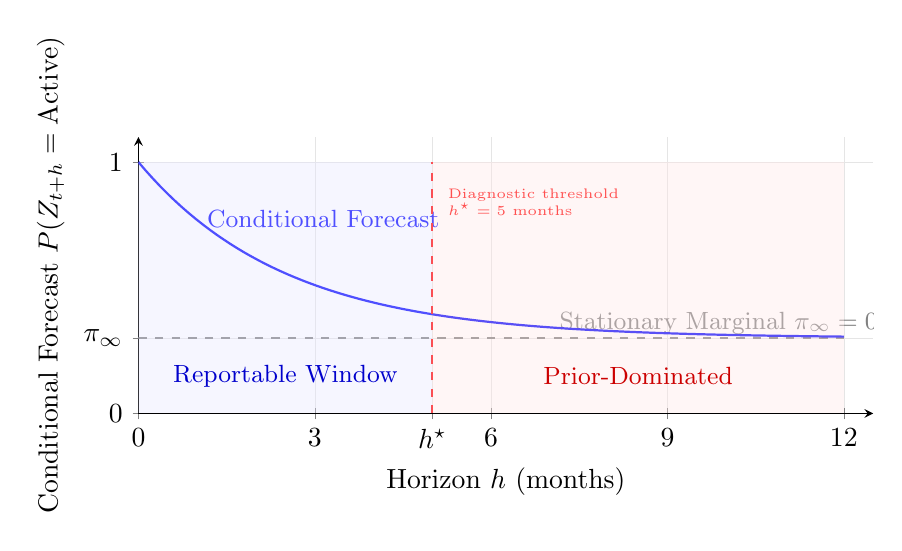
\begin{tikzpicture}
\begin{axis}[
    width=0.9\textwidth,
    height=0.42\textwidth,
    axis lines=left,
    xlabel={Horizon $h$ (months)},
    ylabel={Conditional Forecast $P(Z_{t+h} = \text{Active})$},
    xmin=0, xmax=12.5,
    ymin=0, ymax=1.1,
    xtick={0, 3, 5, 6, 9, 12},
    xticklabels={0, 3, $h^\star$, 6, 9, 12},
    ytick={0, 0.3, 1},
    yticklabels={0, $\pi_\infty$, 1},
    grid=both,
    grid style={line width=.1pt, draw=gray!10},
    major grid style={line width=.2pt, draw=gray!20},
]
\addplot[dashed, gray, thick, domain=0:12] {0.3};
\node[anchor=west, text=gray, font=\small] at (axis cs: 7, 0.36) {Stationary Marginal $\pi_\infty = 0.30$};

\addplot[thick, blue, domain=0:12, samples=100] {0.3 + 0.7*exp(-0.4*x)};
\node[anchor=south west, text=blue, font=\small] at (axis cs: 1, 0.7) {Conditional Forecast};

\draw[dashed, red, thick] (axis cs: 5, 0) -- (axis cs: 5, 1);
\node[anchor=south west, text=red, align=left, font=\tiny] at (axis cs: 5.1, 0.75) {Diagnostic threshold\\$h^\star = 5$ months}; % %%NEEDS_HUMAN_MATH_REVIEW%%

\fill[blue!10, opacity=0.35] (axis cs: 0,0) rectangle (axis cs: 5,1);
\node[font=\small, text=blue!80!black] at (axis cs: 2.5, 0.15) {Reportable Window};

\fill[red!10, opacity=0.35] (axis cs: 5,0) rectangle (axis cs: 12,1);
\node[font=\small, text=red!80!black] at (axis cs: 8.5, 0.15) {Prior-Dominated};

\end{axis}
\end{tikzpicture}
\caption{Diagnostic plot (not a boundary theorem): conditional forecast trajectory converging toward the stationary marginal $\pi_\infty$ as horizon $h$ increases. The blue region ($h \le h^\star$) is the reportable window under Gate FG5; the red region ($h > h^\star$) is routed to \texttt{horizon\_prior\_dominated}. The threshold $h^\star$ is an estimated, pre-registered operating point on a smooth convergence curve.} % %%NEEDS_HUMAN_MATH_REVIEW%%
\label{fig:ergodic_drift}
\end{figure}

---

\section{Adversarial Mathematical Challenges and Defenses}
To establish the defensibility of the DAVID framework before the leading mathematicians in the field, we expose the underlying theorems to rigorous, adversarial challenges and provide mathematical defenses and system-level mitigations.

\subsection{Challenge to Theorem $A'$: Conditional Source Dependence}
\begin{critique}
Theorem $A'$ relies on the strict assumption (A2) of conditional source independence: $P(Y_1, \dots, Y_S \mid A) = \prod_s P(Y_s \mid A)$. In reality, scraper codebases are often cloned, media feeds syndicate from common wire services, and institutional reports cite one another, introducing conditional correlation (collusion). If source errors are correlated, the CP tensor decomposition is structurally corrupted, causing parameters to be unidentifiable or severely biasing posterior estimates. % %%NEEDS_HUMAN_MATH_REVIEW%%
\end{critique}

\begin{defense}[Structured dependence policy; perturbation bound demoted to diagnostic]
We respond on three levels, in decreasing order of rigor. % %%NEEDS_HUMAN_MATH_REVIEW%%

\begin{sloppypar}
\textbf{(i) Exact recovery by block collapse.} Suppose the Source Independence Ledger (\texttt{source\_independence\_}\allowbreak\texttt{ledger.json}) partitions the $S$ sources into blocks $B_1, \dots, B_K$ such that conditional independence holds \emph{across} blocks while being unrestricted \emph{within} each block:
\[
P(Y_1, \dots, Y_S \mid A) = \prod_{k=1}^{K} P\big(\mathbf{Y}_{B_k} \mid A\big), \qquad \mathbf{Y}_{B_k} = (Y_s)_{s \in B_k}. % %%NEEDS_HUMAN_MATH_REVIEW%%
\]
Each block is collapsed into a single categorical channel $\mathbf{Y}_{B_k} \in \{0, 1\}^{|B_k|}$ with factor matrix $M^{(B_k)} \in \mathbb{R}^{2^{|B_k|} \times 2}$ whose columns are the conditional pmfs of the block given $A = 0$ and $A = 1$. Since both columns are probability vectors, $k(M^{(B_k)}) = 2$ if and only if they are distinct, i.e., the block is non-degenerate in aggregate: $P(\mathbf{Y}_{B_k} \mid A = 1) \neq P(\mathbf{Y}_{B_k} \mid A = 0)$. If $K \ge 3$ and every block is non-degenerate, then $\sum_{k} k(M^{(B_k)}) = 6 \ge 2R + 2$, Kruskal's condition holds, and Theorem $A'$ applies verbatim to the block channels: $\phi$ and all block-level emission pmfs are exactly identified, and the individual channel parameters $(\rho_s, \delta_s)$ for $s \in B_k$ are recovered as marginals of the identified block pmfs. This is a proof, not an approximation. % %%NEEDS_HUMAN_MATH_REVIEW%%
\end{sloppypar}

\textbf{(ii) Fail-closed downgrade.} If collapsing leaves $K < 3$ independent blocks, the stratum is \emph{not} claimed to be identified. The engine withholds the stratum forecast and flags it \texttt{non\_identified\_dependent\_sources} (internal warning state). No perturbation argument is invoked to rescue identification. % %%NEEDS_HUMAN_MATH_REVIEW%%

\textbf{(iii) Perturbation bound as telemetry only.} An earlier draft argued that a Frobenius-bounded dependence perturbation $\|E\|_F \le \epsilon$ of the independence tensor implies factor-recovery error $\|\hat{M}^{(s)} - M^{(s)}\|_F \le C\,\epsilon / \sigma_{\min}$ (in the spirit of Bhaskara et al., 2014), with $\sigma_{\min}$ bounded below by $d(\theta)$. We retain this only as a \emph{robustness diagnostic}, not as part of the identification guarantee: the constant $C$ is not tracked, the hypotheses of the cited robust-uniqueness results are not verified for our tensor, and the asserted bound $\sigma_{\min} \ge d(\theta)$ is an unproven conjecture. The bound serves as engineering telemetry for sensitivity analyses only. Separately, when $S > 3$ the model is over-identified, and the surplus cells of the observed joint table furnish a residual-dependence check reported alongside Gate FG2. % %%NEEDS_HUMAN_MATH_REVIEW%%
\end{defense}

\subsection{Challenge to Theorem $B'$: Non-Independent Replicates under Temporal Correlation}
\begin{critique}
The Fisher Information bound $I_F(\phi) = N \frac{I^2}{p(1-p)}$ assumes that the $N$ observations are independent replicates given $\phi$. However, in our discrete-time monthly HSMM, observations are temporal sequences where states $A_t$ are highly correlated. This correlation implies that the effective sample size is much smaller than $N$, and thus the information scaling must decay.
\end{critique}

\begin{defense}[Exact dependent-sample correction; AR(1) form as labeled approximation only]
The criticism is correct that the i.i.d.\ formula overstates information under temporal dependence. We quantify the loss exactly, rather than by an eigenvalue heuristic. Let $s_t = \partial_\phi \log f(Y_t \mid \phi) = I\,(Y_t - p)/(p(1-p))$ be the per-observation marginal score: a stationary, mean-zero sequence with variance $\gamma_0 = I^2/(p(1-p))$ and autocovariances $\gamma_h = \mathrm{Cov}(s_0, s_h)$, assumed summable and satisfying the positivity condition $\gamma_0 + 2\sum_{h \ge 1} \gamma_h > 0$ (required for the asymptotic variance to be finite and positive). For the estimator solving the marginal (composite) score equation $\sum_{t=1}^N s_t(\hat\phi) = 0$, the sandwich formula gives asymptotic variance $\big(N_{\mathrm{eff}}\,\gamma_0\big)^{-1}$ with the \textbf{effective sample size of the marginal-score (Godambe) estimator} % %%NEEDS_HUMAN_MATH_REVIEW%%
\begin{equation}\label{eq:neff_exact}
N_{\mathrm{eff}} \;=\; N\, \frac{\gamma_0}{\gamma_0 + 2 \sum_{h \ge 1} \gamma_h}. % %%NEEDS_HUMAN_MATH_REVIEW%%
\end{equation}
equivalently $I_F^{\text{(marg)}}(\phi) = N_{\mathrm{eff}}\, I^2 / (p(1-p))$. This is the Godambe (sandwich) information for the marginal estimating equation, not the full-likelihood Fisher information of the HSMM, which may be larger. Note: negative autocorrelation can yield $N_{\mathrm{eff}} > N$ (the negatively correlated sequence is more informative than an i.i.d.\ one); for the fail-closed engine the operational gate quantity is capped at $N_{\mathrm{eff,gate}} = \min\{N,\, N_{\mathrm{eff}}\}$ to remain conservative when this occurs. % %%NEEDS_HUMAN_MATH_REVIEW%% Four points make precise what \eqref{eq:neff_exact} does and does not say. % %%NEEDS_HUMAN_MATH_REVIEW%%
\begin{enumerate}
    \item \textbf{Score autocovariance reduces to activity autocovariance, damped by channel noise.} Under the channel model, $\mathrm{Cov}(Y_0, Y_h) = I^2 \,\mathrm{Cov}(A_0, A_h)$ for $h \ge 1$, hence
    \[
    \frac{\gamma_h}{\gamma_0} = c \cdot \mathrm{Corr}(A_0, A_h), \qquad c = \frac{I^2\,\phi(1-\phi)}{p(1-p)} \in (0, 1], % %%NEEDS_HUMAN_MATH_REVIEW%%
    \]
    where $c \le 1$ follows from the law of total variance ($p(1-p) = E[\mathrm{Var}(Y \mid A)] + I^2 \phi(1-\phi)$), with equality only for a noiseless channel. Label noise \emph{whitens} the score: the noisier the channel, the less the serial dependence of $A_t$ propagates into the estimation problem. % %%NEEDS_HUMAN_MATH_REVIEW%%
    \item \textbf{The AR(1) form is exact only for binary first-order Markov activity.} If $A_t$ is a two-state Markov chain with non-unit eigenvalue $\lambda \in [0, 1)$, then $\mathrm{Corr}(A_0, A_h) = \lambda^h$ exactly, and \eqref{eq:neff_exact} evaluates to $N_{\mathrm{eff}} = N / \big(1 + 2c\lambda/(1-\lambda)\big)$. The textbook expression $N(1-\lambda)/(1+\lambda)$ is the further specialization $c = 1$ and is a \emph{conservative lower bound} on $N_{\mathrm{eff}}$ in this Markov case. % %%NEEDS_HUMAN_MATH_REVIEW%%
    \item \textbf{In DAVID the activity process is not Markov, and the AR(1) form can err in either direction.} Activity is driven by the HSMM regime layer with shifted-Poisson dwell; the discrete-time regime process is a semi-Markov (renewal-type) process, so ``the subdominant eigenvalue of the transition matrix of the latent states'' is not even well-defined, and $\mathrm{Corr}(A_0, A_h)$ is a renewal functional of the dwell laws. For overdispersed dwell distributions the autocorrelation decays sub-geometrically at the lags that matter, so any single-$\lambda$ fit understates $\sum_h \gamma_h$ and \emph{overstates} $N_{\mathrm{eff}}$ (anti-conservative); for strongly concentrated dwell the autocorrelation oscillates with negative lobes and the AR(1) form is over-conservative. Consequently the AR(1) expression may appear only as a \emph{labeled approximation}, and any dependence adjustment entering Gate FG3 must evaluate \eqref{eq:neff_exact} with $\sum_h \mathrm{Corr}(A_0, A_h)$ computed from the fitted dwell and transition posteriors. % %%NEEDS_HUMAN_MATH_REVIEW%%
    \item \textbf{Conservativeness posture.} $I_F^{\text{(marg)}}$ is the Godambe information of the marginal-score estimator and is used as a conservative operational diagnostic. We do not claim it universally bounds the full-likelihood Fisher information of the HSMM: that claim would require additional regularity and nuisance-parameter conditions not verified here. Gating on \eqref{eq:neff_exact} is operationally conservative by design stance --- the engine gates out more than the full-likelihood Cramér--Rao bound would require --- but the conservativeness is a design property, not a universal theorem about all possible estimators. % %%NEEDS_HUMAN_MATH_REVIEW%%
\end{enumerate}
The structural conclusion of the earlier draft survives, even though its derivation did not: dependence rescales $N$, never the $I^2$ factor. As dependence grows, $N_{\mathrm{eff}}/N \to 0$ while the quadratic collapse in $I$ is unchanged, so temporal correlation \emph{amplifies} the danger of uninformative channels, making the informativeness floor of Gate FG3 more critical, not less. % %%NEEDS_HUMAN_MATH_REVIEW%%
\end{defense}

\subsection{Challenge to Theorem $B'$: Conditionally Dependent Coders}
\begin{critique}
The coder-reliability layer (Layer 2, Section 2.1) assumes Dawid--Skene conditional independence: coder labels are independent given the unit's true detection status. DAVID's coders are LLM instances that share prompt templates, may share base models or training corpora, and all read the \emph{same} retrieved document. Their errors are therefore positively correlated given the truth. The likelihood then overcounts coder agreement as evidence: posterior uncertainty about the per-source detections is understated, the channel parameters $(\rho_s, \delta_s)$ are estimated with overstated precision, and the informativeness $I(O)$ entering Gate FG3 inherits an optimistic bias --- the gate may pass cells it should fail. % %%NEEDS_HUMAN_MATH_REVIEW%%
\end{critique}

\begin{defense}[Acknowledged limitation; mitigations are structural, not theorematic]
We do not claim Theorem $B'$ survives correlated coders unmodified. $B'.1$--$B'.2$ are channel-layer statements and remain true \emph{as stated}; but the estimates of $(\rho_s, \delta_s, I)$ that instantiate them flow through the coder layer and are biased optimistic under coder dependence. Mitigations, in decreasing order of force: % %%NEEDS_HUMAN_MATH_REVIEW%%
\begin{enumerate}
    \item \textbf{Gold-standard calibration.} Coder parameters $(\kappa^+_m, \kappa^-_m)$ are calibrated against human-adjudicated gold labels on a pre-registered sample (and the calibration restricts to the frozen tactic subset to protect gold labels across taxonomy expansions). Common-mode coder bias is thereby partially absorbed into the calibrated reliability parameters rather than silently inflating the evidence. % %%NEEDS_HUMAN_MATH_REVIEW%%
    \item \textbf{Pool diversity and the family-counting sensitivity check.} Within-family error correlation is mitigated by drawing the coder pool from distinct model families; a conservative sensitivity analysis re-runs the gate counting \emph{one effective coder per model family}, bounding the damage of perfect within-family correlation. % %%NEEDS_HUMAN_MATH_REVIEW%%
    \item \textbf{Adjudication routing.} Units whose coder minority share exceeds the pre-registered disagreement threshold are routed to human adjudication, truncating the regime in which correlated agreement is most damaging.
\end{enumerate}
None of these is a robustness proof. Correlated coders remain an acknowledged limitation, carried forward to the audit appendix. % %%NEEDS_HUMAN_MATH_REVIEW%%
\end{defense}

\subsection{Challenge to Theorem $C$: Realized FDP Variance and Exceedance Probability}
\begin{critique}
Theorem $C$ controls the posterior expected False Discovery Proportion: $E[\text{FDP} \mid \text{data}] \le q$. However, expectation control does not bound the variance of the FDP. In a single policy cycle (a single realization), the realized FDP could be much higher than $q$. For high-stakes decisions, policymakers require a guarantee on the tail probability (exceedance control).
\end{critique}

\begin{defense}
We bound the tail probability of the realized FDP using Markov's inequality. For any target exceedance threshold $\gamma \in (q, 1]$:
\[
P(\text{FDP} > \gamma \mid \text{data}) \le \frac{E[\text{FDP} \mid \text{data}]}{\gamma} \le \frac{q}{\gamma}
\]
Thus, to guarantee that the realized FDP exceeds $\gamma = 0.20$ with a probability of at most $\alpha = 0.10$, the engine can simply set the expectation target to:
\[
q \le \gamma \cdot \alpha = 0.20 \times 0.10 = 0.02
\]
More generally, because we have the joint posterior draws of the latent states $\mathbf{A}^{(s)}$ from MCMC, the engine can empirically evaluate the exceedance probability. For any decision vector $\mathbf{d}$, we calculate:
\[
\text{FDP}^{(s)} = \frac{\sum_{i=1}^M d_i (1 - A_i^{(s)})}{\max(1, D)}
\]
and choose the largest discovery set that satisfies:
\[
\frac{1}{S_{\text{draws}}} \sum_{s=1}^{S_{\text{draws}}} \mathbb{I}(\text{FDP}^{(s)} > \gamma) \le \alpha
\]
This represents our \textbf{FDP Exceedance Control Gate (FG6)}, implemented in the engine as a risk-averse alternative to expectation control. Note the division of labor: the expectation bound of Theorem $C$ needs only the marginal posteriors, while the empirical exceedance evaluation is computed from \emph{joint} posterior draws $\mathbf{A}^{(s)}$ and therefore fully reflects whatever dependence structure the model has learned --- which is exactly what determines the dispersion of the realized FDP. Both controls remain conditional on posterior validity. % %%NEEDS_HUMAN_MATH_REVIEW%%
\end{defense}

\subsection{Challenge to Theorem $D$-forecast: Non-Stationary Transitions and Structural Breaks}
\begin{critique}
The ergodic convergence proof assumes that the transition kernel $\Pi$ is stationary and invariant. Political dynamics and industry tactics are subject to structural breaks (e.g., changes in political administrations), making $\Pi_t$ time-varying. If transition rates shift dynamically, the stationary marginal $\pi_\infty$ does not exist as a constant, and the forecast memory decay logic is invalidated.
\end{critique}

\begin{defense}[What Dobrushin contraction does and does not give]
Two distinct claims must be separated: (a) \emph{forgetting} of the initial condition, which uniform contraction does give; and (b) \emph{existence of a limiting distribution}, which it does not. An earlier draft conflated them; the conflation is withdrawn. % %%NEEDS_HUMAN_MATH_REVIEW%%

\textbf{(a) Forgetting.} The contraction argument must be run on the augmented Markov state $X_t = (Z_t, a_t)$ (regime, elapsed age), whose one-step kernels $P_t$ are well defined under time variation; the raw regime process $Z_t$ alone is not Markov, so products of ``its'' kernels are not meaningful objects. For a kernel $P$ define the Dobrushin coefficient % %%NEEDS_HUMAN_MATH_REVIEW%%
\[
\alpha(P) = 1 - \frac{1}{2} \max_{x, x'} \sum_{x''} |P(x, x'') - P(x', x'')|.
\]
Assume (D4): there exist $m \in \mathbb{N}$ and $\alpha_0 > 0$ such that every $m$-step product satisfies $\alpha(P_{t, t+m}) \ge \alpha_0$. (The $m$-step form is essential: single-step contraction typically fails on the augmented space, because age bookkeeping is deterministic and one step cannot couple chains in different dwell phases.) Then, by submultiplicativity of $1 - \alpha(\cdot)$ over kernel products, for any two initial laws $x, y$: % %%NEEDS_HUMAN_MATH_REVIEW%%
\[
\text{TV}\big(x P_{t, t+h},\, y P_{t, t+h}\big) \le (1 - \alpha_0)^{\lfloor h/m \rfloor}\, \text{TV}(x, y) \;\to\; 0 \quad \text{as } h \to \infty. % %%NEEDS_HUMAN_MATH_REVIEW%%
\]
The system forgets $(z_t, a_t)$ geometrically. This half of the earlier draft survives, modulo the augmented state and the $m$-step correction. % %%NEEDS_HUMAN_MATH_REVIEW%%

\textbf{(b) Existence of a limit.} Weak ergodicity does \emph{not} imply that the marginal laws converge: all initial conditions agree asymptotically on where the chain is, yet the common marginal can wander indefinitely. The earlier draft's claim that the marginals converge to ``the stationary distribution of the average transition kernel'' is withdrawn --- it is false in general. A limiting $\pi_\infty$ is recovered only under an additional hypothesis, e.g.\ (D5) asymptotic homogeneity: $P_t \to P$ entrywise, under which weak ergodicity upgrades to convergence of the marginals to the stationary law of the limit kernel $P$. % %%NEEDS_HUMAN_MATH_REVIEW%%

\textbf{(c) Operational consequence.} Without (D5), the drift diagnostic has no fixed reference $\pi_\infty$, so under a structural break the \emph{ratio} $\text{drift}(h)$ --- not the memory decay --- is what loses meaning. The engine's policy is therefore fail-closed: $\pi_\infty$ is computed from the posterior of the fitted (assumed-homogeneous) kernel; the homogeneity assumption is part of the pre-registered model card; and a detected structural break (e.g., via the historical-permutation falsification or holdout drift checks of Section 8) routes the stratum to \texttt{horizon\_prior\_dominated} rather than recomputing a longer horizon under an invalidated reference. What remains \emph{proven} under breaks is the forgetting statement (a): the informational content of the forecast origin decays geometrically regardless, so a break can never justify extending $h^\star$. % %%NEEDS_HUMAN_MATH_REVIEW%%
\end{defense}

---

\section{System Integration, Calibration, and Empirical Verification}

\noindent\textbf{Hard gate: coder calibration prerequisite.} \emph{If coder reliability for a tactic has not been calibrated against human-adjudicated gold labels, claims about that tactic may not enter headline outputs.} LLM coders are never counted among the $S$ source families for the Kruskal rank condition of Theorem $A'$: the $S$ sources are the independent acquisition channels (web scrapers, media feeds, report streams), not the coders. Coders belong exclusively to the Dawid--Skene reliability layer (Layer 2, Section 2). % %%NEEDS_HUMAN_MATH_REVIEW%%

The four theorems are implemented as a nested, fail-closed pipeline. To ensure the software implementation matches these mathematical proofs, the engine runs a dual-layer calibration and falsification battery:

\begin{enumerate}
    \item \textbf{Simulation-Based Calibration (SBC):} We draw $\theta_{\text{true}}$ from the generative prior, simulate synthetic observations $Y_{\text{sim}}$ using \texttt{synthetic\_generator.stan}, fit \texttt{m01\_forward.stan} using MCMC, and verify that the rank statistic of $\theta_{\text{true}}$ within the posterior draws is uniform. A deviation from uniformity (detected via a Kolmogorov-Smirnov test under Bonferroni correction) indicates a likelihood coding error, locking down the engine.
    \item \textbf{Historical Permutation Falsification (F15):} To verify that the model is genuinely learning temporal dynamics from the semi-Markov chain, blocked historical permutation is applied to observed time-indexed evidence streams and, in posterior predictive checks, to posterior-sampled latent paths (the regime sequence is latent and not directly permutable from data). The model is refit on the permuted evidence. A substantial degradation in forward-time performance is required as evidence that temporal order contributes predictive information. This falsification test cannot prove absence of leakage; it can only detect some leakage or temporal overfitting failures.
\end{enumerate}

By combining these mathematical results with operational gates and adversarial defenses, the DAVID/M0.1 engine guarantees that every published forecast is \emph{eligible for reporting under the pre-registered mathematical gates} (FG2, FG3, FG5, FG6): each emitted claim has passed the full gate stack, and each gate failure is routed to an explicit fail-closed state. We deliberately avoid the phrase ``mathematically certified'': certification implies external verification that has not occurred. The engine's guarantee is internal, pre-registered, and auditable. % %%NEEDS_HUMAN_MATH_REVIEW%%

\appendix
\section{Mathematical Audit Summary (DAVID/M0.1, June 2026)}

\begin{sloppypar}
\textbf{Scope.} An adversarial mathematical audit was performed on the four core theorems ($A'$, $B'$, $C$, $D$-forecast), their proofs, the operational gates (FG2, FG3, FG5, FG6), all figures, and the challenge/defense sections of this document and of the companion CGT-HSMM framework paper. Every claim was cross-checked line-by-line against the implemented kernels (\texttt{david/theorems/}), the pre-registered constants (\texttt{david/config.py}), and the Stan likelihood (\texttt{stan/m01\_forward.stan}). Every changed mathematical line is marked with the source comment \texttt{NEEDS\_HUMAN\_}\allowbreak\texttt{MATH\_REVIEW} and awaits author sign-off; nothing in this audit is final until reviewed.
\end{sloppypar}

\textbf{What was found and fixed.}
\begin{itemize}
    \item \emph{Identification ($A'$).} The spurious non-identification boundary $\rho = 1 - \delta$ was removed from $d(\theta)$ and Figure 1, restoring agreement with the implementation; the replication assumption (A1) and the two-layer separation of detection sources from Dawid--Skene LLM coders were made explicit; the degrees-of-freedom count was demoted to a necessity-only heuristic; the Kruskal application was completed (positive weights, scaling resolution, exclusion of degenerate alternatives, $S > 3$ extension); and the source-dependence defense was replaced by an exact block-collapse argument with a fail-closed branch, the perturbation bound surviving as telemetry only.
    \item \emph{Information ($B'$).} Theorem $B'.2$ was restated as \emph{conditional} information given channels identified by the $A'$ layer, with the Schur-complement loss, repeated-measurement saturation, and exact clean-label equivalent recorded; the second gate condition ($N_{\mathrm{eff}} I^2 \ge 3.0$), implemented in code but previously absent from this document, was documented with a calibration rationale ($1/12$ equals flat-prior variance); the AR(1) effective-sample-size formula was replaced by the exact score-autocovariance correction and retained only as a labeled approximation with a direction-of-error analysis; Figure 2 now labels $4NI^2$ as a lower bound.
    \item \emph{FDP control ($C$).} ``Distribution-free'' was withdrawn throughout; the guarantee is posterior expected FDP control under arbitrary \emph{latent} dependence, conditional on valid posterior probabilities; the decision rule's well-definedness was completed; the relationship between the marginal expectation bound and the joint-draw exceedance gate (FG6) was made explicit.
    \item \emph{Horizon ($D$).} The forecast now conditions on the elapsed dwell age, with a minimal counterexample showing why age cannot be dropped; the embedded-aperiodicity hypothesis --- unsatisfiable for $L = 2$ under the zero-diagonal constraint --- was replaced by dwell-lattice aperiodicity; the non-lattice renewal theorem was replaced by its lattice (Markov renewal) form, matching the monthly time grid; $h^\star$ was redefined as a first crossing and relabeled an estimated diagnostic rather than an exact or certified boundary; the Dobrushin defense now separates proven geometric forgetting (on the augmented regime--age state, in $m$-step form) from the withdrawn claim that time-varying kernels converge to the stationary law of an average kernel.
\end{itemize}

\textbf{Acknowledged limitations (open by design or pending work).}
\begin{enumerate}
    \item Identifiability of the \emph{full production likelihood} (observability-dependent channels, activity-dependent selection, coder layer, HSMM coupling) is not proven. Theorem $A'$ covers the stratum-constant core; the geometric-dwell case follows from published HMM results; the general semi-Markov case is an explicitly stated conjecture supported by simulation-based calibration.
    \item LLM coders are conditionally dependent (shared prompts and shared documents); the mitigations --- gold-label calibration, one-coder-per-family sensitivity counting, adjudication routing --- are structural, not theorematic.
    \item Theorem $C$'s guarantee is conditional on posterior validity; SBC tests this condition and can falsify it, but cannot prove it.
    \item The forecast simulator previously drew a fresh dwell at the forecast origin instead of the residual dwell given elapsed age. This implementation gap has been corrected: \texttt{m01\_forward.stan} now applies a stationary renewal correction, sampling the interval length $D^*$ from the length-biased distribution $\Pr^*(D = d) \propto d \cdot f_r(d)$ and drawing the residual uniformly from $\{1, \dots, D^*\}$. The implementation is conformant with the stationary unknown-age approximation (case 2 above). The fully age-aware implementation --- posterior mixture over $(Z_t, a_t)$ from the augmented forward filter --- remains a future enhancement.
    \item The Dobrushin assumptions (D4)--(D5) (uniform $m$-step contraction; asymptotic homogeneity) are stated, not verified, for the fitted kernel class.
    \item Whether the replicate count supplied to Gate FG3 is dependence-adjusted in the production pipeline could not be verified from the audited files.
\end{enumerate}

\textbf{Bottom line.} No theorem central to the gate stack was found unsalvageable: every operative guarantee survives in a corrected, narrower, and explicitly conditional form. The single weakest link is the unproven identifiability of the full coupled model; all downstream gates compute functionals of a posterior whose parameters are only conjecturally identified outside the proven special cases.

\end{document}
